\documentclass[10pt,twocolumn,letterpaper]{article}

\usepackage[margin=0.75in]{geometry}
\usepackage{times}
\usepackage{graphicx}
\usepackage{amsmath}
\usepackage{amssymb}
\usepackage{booktabs}
\usepackage{multirow}
\usepackage{array}
\usepackage{xcolor}
\usepackage{hyperref}
\usepackage{enumitem}
\usepackage{caption}
\usepackage{subcaption}
\usepackage{url}
\usepackage{placeins}
\usepackage{dblfloatfix}
\usepackage{float}

\graphicspath{{../}}
\hypersetup{colorlinks=true, linkcolor=blue, citecolor=blue, urlcolor=blue}
\captionsetup{font=small,labelfont=bf}
\setlength{\textfloatsep}{8pt plus 2pt minus 2pt}
\setlength{\floatsep}{6pt plus 2pt minus 2pt}
\setlength{\intextsep}{6pt plus 2pt minus 2pt}
\setlength{\abovecaptionskip}{4pt}
\setlength{\belowcaptionskip}{0pt}
\emergencystretch=2em
\raggedbottom

\newcommand{\todo}[1]{\textcolor{red}{[TODO: #1]}}
\newcommand{\figpath}[1]{{\scriptsize\path{#1}}}

\title{Multi-source 3D Asset Generation and Real-scene Fusion with 2D Gaussian Splatting and AIGC}

\author{
  \textbf{[Name Placeholder]} \\
  Student ID: \textbf{[Student ID Placeholder]} \\
  GitHub: \url{[GitHub Repository URL Placeholder]} \\
  ModelScope / Weights: \url{[ModelScope Link Placeholder]}
}
\date{}

\begin{document}
\maketitle

\begin{abstract}
This report documents a two-task computer vision assignment under a shared 3D vision and generative modeling theme.
The current draft completes Task 1: three assets are generated from real multi-view reconstruction, text-to-3D synthesis, and single-image-to-3D reconstruction, then inserted into a real scene reconstructed by 2D Gaussian Splatting (2DGS).
The background is the Mip-NeRF 360 garden scene, selected from a 5k/15k/30k 2DGS ablation.
Object A is reconstructed from a phone video through COLMAP and 2DGS, Object B is generated by SDS-based text-to-3D optimization in threestudio, and Object C is generated from one image with background removal and Magic123.
The final video uses a synchronized rendering pipeline: 2DGS renders a 900-frame background trajectory and exports the same camera sequence to Blender, where the A/B/C meshes are rendered as transparent foreground and composited with RGB/depth-aware masks.
The final Task 1 artifact is a 15-second, 900-frame, 1080p, 60fps multi-view video.
The experiments show that the three asset routes fail differently: multi-view reconstruction is strongest before mesh export, text-to-3D is flexible but prior-driven, and single-image reconstruction preserves front-view detail but hallucinates unobserved geometry.
\end{abstract}

\section{Introduction}
Task 1 asks for a complete real-scene fusion pipeline rather than a single reconstruction result.
The background must come from a real open-source scene reconstructed by 2DGS; the three objects must come from three different sources; and the final output must be a multi-view walkthrough video with all assets fused into one scene.
The assignment therefore tests not only reconstruction quality, but also the engineering and geometric consistency of the whole pipeline.

The three inserted assets have incompatible assumptions.
Object A is grounded in real multi-view images, but the 2DGS representation must be converted into a mesh before Blender rendering.
Object B is produced from a text prompt, so its shape and texture come from an SDS prior rather than real observations.
Object C is constrained by one image, so its front appearance is reliable while its side and back geometry are inferred.
The garden background has its own COLMAP/2DGS coordinate system.
The final fusion must therefore handle different axes, scales, origins, object qualities, and camera models.

Several early fusion previews exposed why a naive solution is insufficient.
A fixed 2DGS backplate preserved the garden appearance but did not provide convincing viewpoint motion.
A proxy Blender garden preserved object parallax but distorted the background into image panels.
A moving-background composite changed the garden view, but the foreground and background cameras were not synchronized.
The final pipeline fixes this by rendering the background and foreground under the same 900-frame pinhole camera sequence.

Task 1 makes four concrete contributions:
\begin{itemize}[leftmargin=*,noitemsep]
    \item a full multi-source asset pipeline covering real multi-view reconstruction, text-to-3D, and single-image-to-3D;
    \item a measured background 2DGS ablation, where the 30k garden checkpoint is selected by PSNR, SSIM, and LPIPS;
    \item a synchronized 2DGS-camera and Blender-foreground compositing pipeline for a 900-frame final video;
    \item a data-backed comparison of the three generation routes, including geometry, texture, compute time, and distortion type.
\end{itemize}

\section{Method}

\subsection{Task 1: Multi-source Asset Generation and Real-scene Fusion}
\paragraph{Background.}
The background is the garden scene from Mip-NeRF 360.
It is reconstructed with 2DGS at three training budgets: 5k, 15k, and 30k iterations.
The 30k checkpoint is used in the final video because it has the best held-out metrics: PSNR 26.6501, SSIM 0.8337, and LPIPS 0.1638.

\paragraph{Object A.}
Object A is captured with a phone video.
Frames are sampled at sparse, medium, and dense rates for COLMAP.
Dense sampling gives the strongest reconstruction, registering 148/148 images with 24125 sparse points and 1.1296 px mean reprojection error.
The dense COLMAP scene is trained with 2DGS for 15000 iterations at half resolution.
The selected run reaches PSNR 24.7654, SSIM 0.8228, and LPIPS 0.3000.

\paragraph{Object B.}
Object B is generated in threestudio using SDS-based text-to-3D optimization.
Three prompt variants are tested.
The selected style-constrained prompt produces the cleanest mug silhouette and the most stable handle/body structure.
The exported mesh has 39314 vertices, 78628 faces, and a 1024$\times$1024 texture.

\paragraph{Object C.}
Object C is generated by Magic123 from a single image.
The first input is a toy-like object, with preprocessing ablated over raw image, automatic background removal, and refined mask.
This first round is later rejected after multi-view inspection: the front view is recognizable, but side/back geometry is unstable and the fused object reads as a blob rather than a reliable 3D asset.
To keep the single-image-to-3D requirement while reducing shape ambiguity, the final Object C is rerun with a simpler mouse image and automatic background removal.
The replacement mesh has 23019 vertices, 46038 faces, and a 2048$\times$2048 albedo texture.

\paragraph{Fusion.}
The final scene keeps A/B/C as textured meshes while the garden remains a separately rendered 2DGS scene.
Each object is first placed by unprojecting a table pixel from 2DGS depth into the garden coordinate system.
Because the source asset axes and geometry are unreliable, the final pose is selected by constrained enumeration over scale, rotation, and height, supported by short rendered previews.
The final video uses a 900-frame 2DGS trajectory, exported as \texttt{cameras\_900.json}, to drive both the 2DGS background renderer and the Blender foreground renderer.
Depth-aware compositing then merges RGB background, background depth, foreground RGBA, and approximate foreground depth.

\subsection{Task 2: Placeholder}
Task 2 will be added after its implementation.
The report structure is reserved so Task 2 can be inserted without changing the Task 1 narrative.
\todo{Add Task 2 method.}

\section{Experiments: Task 1}

\subsection{Background Reconstruction}
The background study is the cleanest ablation because the garden scene has held-out views.
Table~\ref{tab:bg_ablation} shows that every metric improves from 5k to 30k iterations.
The improvement is not cosmetic: LPIPS drops from 0.2556 to 0.1638, and the preview images in Fig.~\ref{fig:bg_ablation} show sharper table boundaries and more stable vegetation texture.
The 30k model is therefore used for all final fusion and video rendering.
The three runs also give a useful estimate of the quality-time trade-off.
The 5k run reaches a plausible reconstruction quickly, but the held-out table edges and grass regions remain perceptually unstable.
The 15k run improves PSNR by 1.0155 dB over 5k and reduces LPIPS by 0.0744, which is the largest single jump in the ablation.
The 30k run gives a smaller PSNR gain over 15k, but it still improves all metrics and produces the most stable final background for compositing.
Since the final video uses the background for every frame, even small residual vegetation or table artifacts are amplified by camera motion; for this reason the final selection favors the best-quality 30k checkpoint rather than the cheaper 15k checkpoint.

\begin{table}[t]
\centering
\caption{Garden 2DGS ablation. The 30k checkpoint is selected.}
\label{tab:bg_ablation}
\begin{tabular}{lccc}
\toprule
Iterations & PSNR$\uparrow$ & SSIM$\uparrow$ & LPIPS$\downarrow$ \\
\midrule
5k  & 25.1907 & 0.7677 & 0.2556 \\
15k & 26.2062 & 0.8209 & 0.1812 \\
30k & \textbf{26.6501} & \textbf{0.8337} & \textbf{0.1638} \\
\bottomrule
\end{tabular}
\end{table}

\begin{figure}[t]
\centering
\begin{subfigure}{0.32\linewidth}
  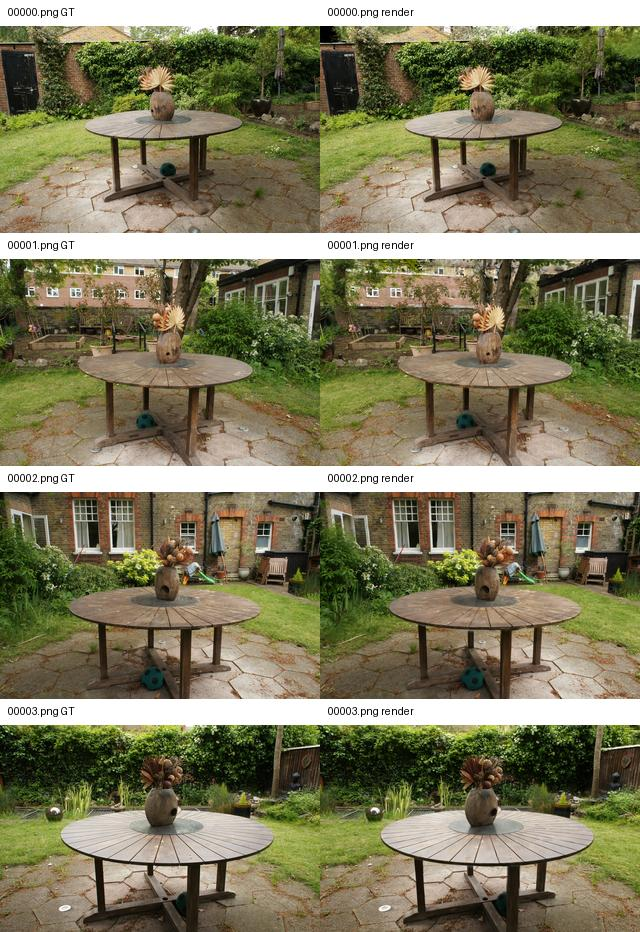
\includegraphics[width=\linewidth]{reports/figures/background_2dgs_low_preview.jpg}
  \caption{5k}
\end{subfigure}
\begin{subfigure}{0.32\linewidth}
  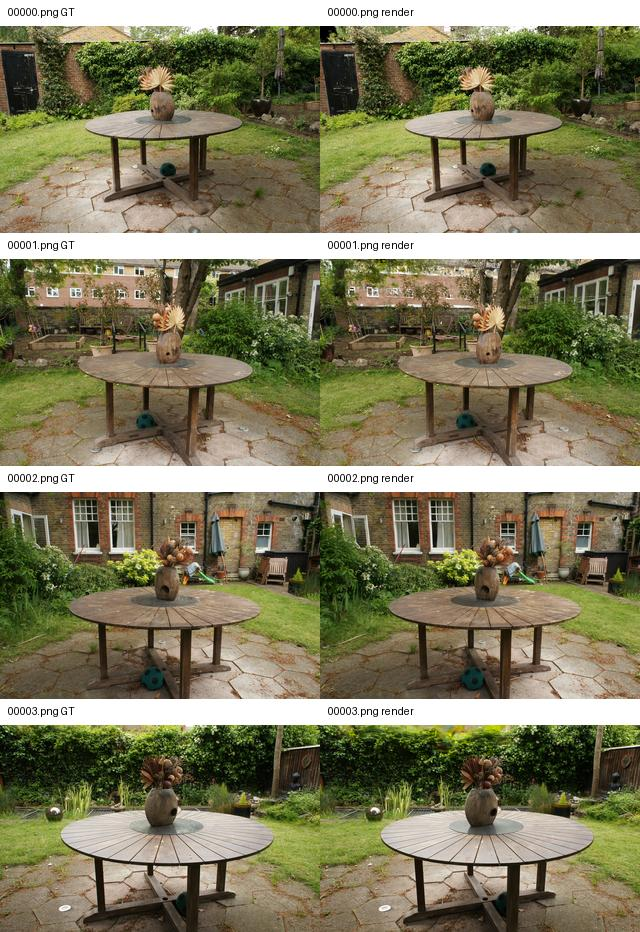
\includegraphics[width=\linewidth]{reports/figures/background_2dgs_mid_preview.jpg}
  \caption{15k}
\end{subfigure}
\begin{subfigure}{0.32\linewidth}
  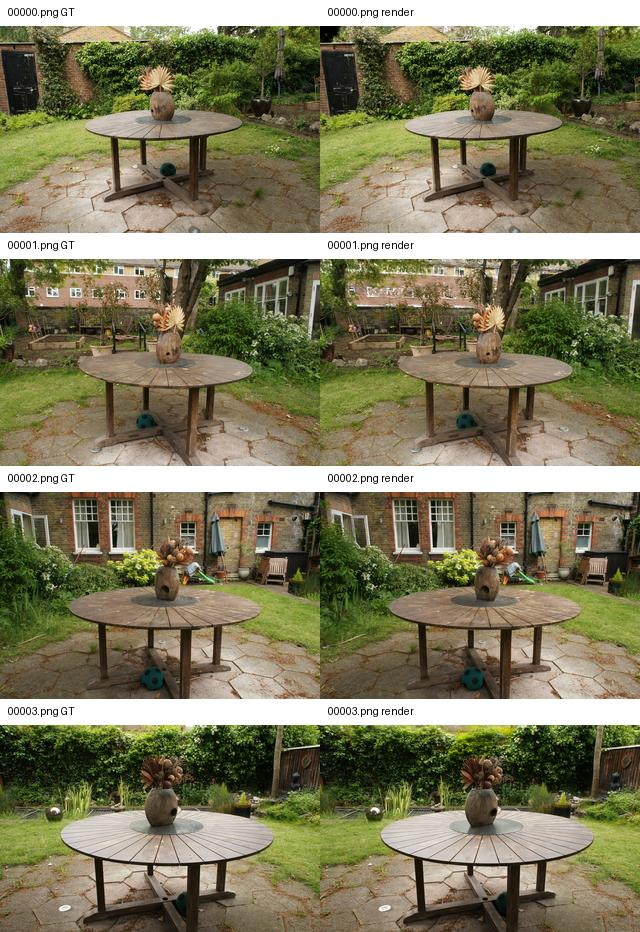
\includegraphics[width=\linewidth]{reports/figures/background_2dgs_high_preview.jpg}
  \caption{30k}
\end{subfigure}
\caption{Background 2DGS previews. The final 30k model gives the most stable table and garden reconstruction among the tested budgets.}
\label{fig:bg_ablation}
\end{figure}

The visual comparison supports the metric trend.
The 5k preview is already recognizable, but the tabletop boundary and nearby grass have weaker structure.
The 15k preview is cleaner and is already usable for a still image.
The 30k model gives the best contact surface for object insertion because the table and its surrounding garden remain sharper under novel views.
This matters for fusion: the inserted A/B/C objects are judged against the table plane, so an unstable background would make correct object scale and contact harder to evaluate.
The final trajectory therefore renders the 30k model for 900 frames rather than reusing a sparse set of 24 evaluation views.

\subsection{Object A: Multi-view Reconstruction}
Object A has the strongest real-image evidence, but it also shows the clearest representation-conversion failure.
Table~\ref{tab:object_a_sampling} compares the COLMAP frame sampling results.
Dense sampling is chosen because it registers every image and gives the largest point cloud.
Table~\ref{tab:object_a_2dgs} then shows the 2DGS resolution and source ablation.
The dense-half rerun is the final choice because it improves PSNR and LPIPS over the earlier full/half medium-source runs.
The dense frame set is not selected simply because it contains more images.
The important signal is that dense sampling registers all 148 input frames and increases the sparse point count from 9837 in the medium run to 24125.
The reprojection error rises only slightly compared with medium, from 1.1265 px to 1.1296 px, while the number of observations and track connectivity increase substantially.
This indicates that the dense set adds useful coverage instead of merely adding noisy frames.

\begin{table}[t]
\centering
\caption{Object A frame sampling and COLMAP reconstruction.}
\label{tab:object_a_sampling}
\begin{tabular}{lrrrr}
\toprule
Set & Frames & Reg. & Points & Reproj. \\
\midrule
Sparse & 49  & 35  & 4130  & 0.9727 \\
Medium & 99  & 87  & 9837  & 1.1265 \\
Dense  & 148 & 148 & 24125 & 1.1296 \\
\bottomrule
\end{tabular}
\end{table}

\begin{table}[t]
\centering
\caption{Object A 2DGS evaluation. Dense-half is selected.}
\label{tab:object_a_2dgs}
\begin{tabular}{lccc}
\toprule
Run & PSNR$\uparrow$ & SSIM$\uparrow$ & LPIPS$\downarrow$ \\
\midrule
Full & 21.8139 & \textbf{0.8420} & 0.3549 \\
Half & 22.4246 & 0.7944 & 0.3245 \\
Dense-half & \textbf{24.7654} & 0.8228 & \textbf{0.3000} \\
\bottomrule
\end{tabular}
\end{table}

The resolution ablation shows a different trade-off.
The full-resolution medium-source run has the highest SSIM, but its PSNR and LPIPS are worse than the half-resolution run.
The final dense-half run improves PSNR to 24.7654 and LPIPS to 0.3000, which makes it the strongest candidate for final fusion.
The result is also consistent with visual inspection: more COLMAP coverage is more valuable for Object A than preserving the full input resolution, because the object has difficult geometry and several low-texture surfaces.
The dense-half setting therefore becomes the selected Object A representation.

\begin{figure}[t]
\centering
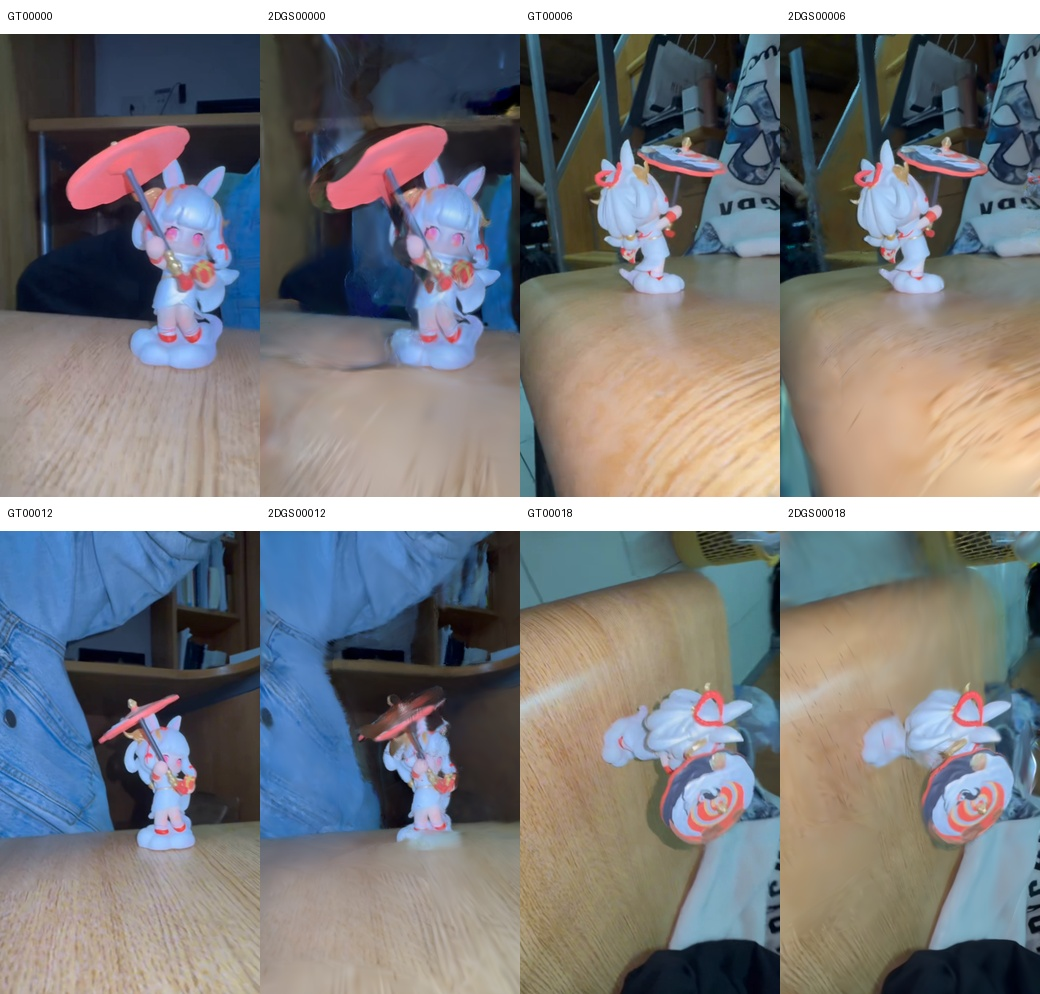
\includegraphics[width=\linewidth]{reports/figures/object_a_2dgs_render_gt_samples.jpg}
\caption{Object A held-out render/GT evidence. Image-space 2DGS rendering preserves recognizable color and view-dependent appearance; the later fusion artifacts are mainly introduced during mesh export.}
\label{fig:object_a_render_gt}
\end{figure}

However, Object A is not a clean success case.
The evidence separates two stages that would otherwise be conflated.
At the image-rendering stage, the dense-half 2DGS model preserves recognizable color and view-dependent appearance.
At the mesh-export stage, the representation becomes much less reliable: the high-resolution mesh export contains 12.27M vertices and 23.78M faces, but much of that geometry is table/background shell rather than object surface.
The lower-resolution mesh is manageable but still requires connected-component filtering; the final selected component has 19922 vertices and 38636 faces.
Thus the final paper should not claim that multi-view reconstruction is artifact-free.
Its advantage is real camera and texture evidence; its weakness in this pipeline is conversion from neural splats to a clean object mesh.

\subsection{Object B and Object C: AIGC Asset Generation}
Object B and C do not have ground-truth multi-view images, so their selection uses a fixed rubric for geometry, texture, fusion readiness, and artifacts.
Table~\ref{tab:b_prompt} shows the SDS prompt ablation.
The style-constrained prompt is selected because it has the best fusion score and lowest Janus artifact risk.
Table~\ref{tab:c_mask} shows the Magic123 mask ablation.
The first-round auto-mask variant initially looked best among raw, automatic, and refined masks, but later multi-view inspection rejected all three first-round C meshes.
The important point is that the AIGC experiments are not judged by a single final screenshot.
For Object B, the prompt affects both geometry and export stability.
For Object C, the mask affects both texture contamination and the inferred 3D shape, but even a clean mask cannot observe the hidden back and side surfaces.
The fixed rubric therefore records geometry, texture, fusion readiness, and artifact notes separately.

\begin{table}[t]
\centering
\caption{Object B prompt ablation. Scores are on a 1--5 rubric.}
\label{tab:b_prompt}
\begin{tabular}{lrrrr}
\toprule
Prompt & Time & Vert. & Geo & Fusion \\
\midrule
Simple & 49:41 & 33999 & 3 & 3 \\
Detailed & 50:03 & 3560 & 2 & 2 \\
Style-constr. & \textbf{47:39} & 39314 & \textbf{4} & \textbf{4} \\
\bottomrule
\end{tabular}
\end{table}

The Object B prompt ablation shows that a longer or more descriptive prompt is not automatically better.
The simple prompt produces a recognizable mug with richer color, but it also produces fuzzier surface structure and ghosting.
The detailed prompt explicitly asks for clean topology and stable proportions, yet the final mesh has only 3560 vertices and receives the lowest geometry and fusion scores.
The style-constrained prompt is selected because it suppresses common SDS failure modes: extra objects, text, faces, and implausible shape.
Its texture remains relatively neutral, but the handle/body silhouette is more stable and therefore more useful for tabletop fusion.
This is why the selected B run prioritizes fusion readiness over visual richness.

\begin{table}[t]
\centering
\caption{Object C Magic123 mask ablation. Scores are on a 1--5 rubric.}
\label{tab:c_mask}
\begin{tabular}{lrrrr}
\toprule
Input & Time & Vert. & Tex & Fusion \\
\midrule
Raw & 16.86m & 18695 & 2 & 1 \\
Auto mask & \textbf{16.72m} & 25874 & 2 & 1 \\
Refined & 17.87m & 27090 & 2 & 1 \\
\bottomrule
\end{tabular}
\end{table}

The Object C ablation gives a different lesson.
The raw image keeps the most unprocessed input information, but the generated texture and silhouette suffer from background pollution.
The refined mask looks cleaner as a 2D input, but in the 3D output it produces more inflated side geometry and fragmented texture.
The automatic mask preserves the front-facing toy appearance best, so it was the best first-round candidate, but the 50 validation views show that this is not a stable 3D reconstruction.
The side and back views are hallucinated, the albedo atlas is fragmented, and the fused result becomes a yellow blob on the garden table.
This failure is stronger than a minor artifact; it is a single-image observability limit.
The final C branch therefore uses a simpler mouse image, whose single-view silhouette is less ambiguous and whose fused preview has clearer object identity.
Even this replacement is treated conservatively: it is scaled and oriented to expose its reliable oblique-front appearance, not claimed as a fully measured 3D object.

\begin{figure}[t]
\centering
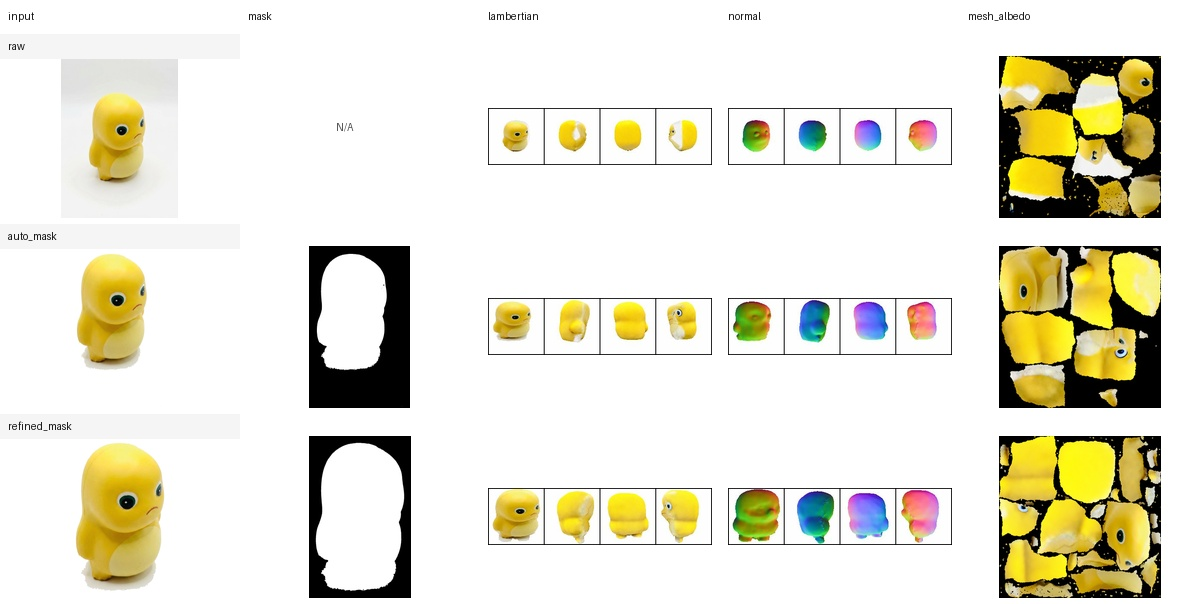
\includegraphics[width=\linewidth]{reports/figures/object_c_magic123_r5_contact_sheet.jpg}
\caption{First-round Object C single-image-to-3D ablation. Auto-mask is the best of the three masks in the front view, but the run is later rejected because side/back validation views do not form a reliable 3D object.}
\label{fig:c_r5_body}
\end{figure}

Together, B and C show two different kinds of generative uncertainty.
Text-to-3D has no real input geometry, so it can create a plausible but prior-driven object whose pose and fine details are arbitrary.
Single-image-to-3D has one real view, so the front texture is more anchored, but all hidden surfaces are inferred.
These differences are why the final fusion does not treat B and C as equally reliable meshes.
B can be rotated into a plausible mug-like tabletop pose; C must be simplified, scaled, and positioned conservatively so that generated side/back structure does not dominate the final video.
Appendix~C gives the detailed C rejection evidence and the mouse-C replacement comparison.

\subsection{Fusion and Final Video}
Fusion required more than importing meshes into Blender.
The first still/video previews exposed incorrect object orientation, missing contact, static backplates, and camera mismatch.
The final scene freezes the user-tuned transforms after many short previews.
Table~\ref{tab:frozen_pose} lists the final transform parameters.
The final video is rendered at 1920$\times$1080, 60 fps, 900 frames, and 15 seconds.
It uses 900 2DGS RGB frames, 900 2DGS depth frames, and 900 Blender foreground frames.
This section is the main engineering result of Task 1.
Early fusion attempts failed for different reasons.
A fixed 2DGS background preserved image quality but made the final video look static.
A proxy Blender environment gave correct foreground parallax, but the garden background became a distorted image-panel approximation.
A moving-background composite gave camera motion, but foreground and background did not share a camera model.
The final synchronized pipeline fixes the most important of these problems by using the same 2DGS camera JSON for both the background trajectory and the Blender foreground render.

\begin{table}[t]
\centering
\caption{Final frozen object transforms in the synchronized scene.}
\label{tab:frozen_pose}
\begin{tabular}{lccc}
\toprule
Obj. & Scale & Rotation $(x,y,z)$ & Location $(x,y,z)$ \\
\midrule
A & 0.735 & $(-30,270,-8)$ & $(-0.40,1.57,0.29)$ \\
B & 0.455 & $(310,10,12)$ & $(0.36,1.80,-0.08)$ \\
C & 0.545 & $(90,-20,4)$ & $(0.99,1.64,0.20)$ \\
\bottomrule
\end{tabular}
\end{table}

The final transform values should be read as the result of constrained search, not as arbitrary manual placement.
The initial object locations come from 2DGS depth unprojection at table pixels A=(610,480), B=(815,500), and C=(990,480).
The subsequent search changes scale, rotation, and height because the asset coordinate systems are inconsistent and the generated meshes are imperfect.
In particular, Object A's mesh component has incomplete surfaces, Object B has arbitrary text-to-3D orientation, and Object C has inferred single-image geometry.
Solving one clean linear transform is not well posed without reliable 3D correspondences, so short preview renders are used to select a visually stable pose.
Shadow provenance is also separated carefully.
Before entering Blender, none of A/B/C carries an independent physical cast-shadow layer.
Object A may contain baked capture illumination or self-shading in its 2DGS colors, Object B's SDS preview contains renderer-dependent shading, and Object C has Magic123 lambertian/albedo outputs, but these are texture or preview effects rather than scene-level shadows.
The contact shadows in the final composite are generated inside Blender by the shared area light and shadow receiver, then composited with the 2DGS garden frames.
To avoid double shadows, the final synchronized render uses a transparent Blender foreground pass and a single 2DGS RGB/depth background pass.
The garden background never contains A/B/C, so there is no pre-existing A/B/C cast shadow to duplicate; the only deliberate object-ground shadow is the Blender-generated contact shadow.

\begin{figure*}[!t]
\centering
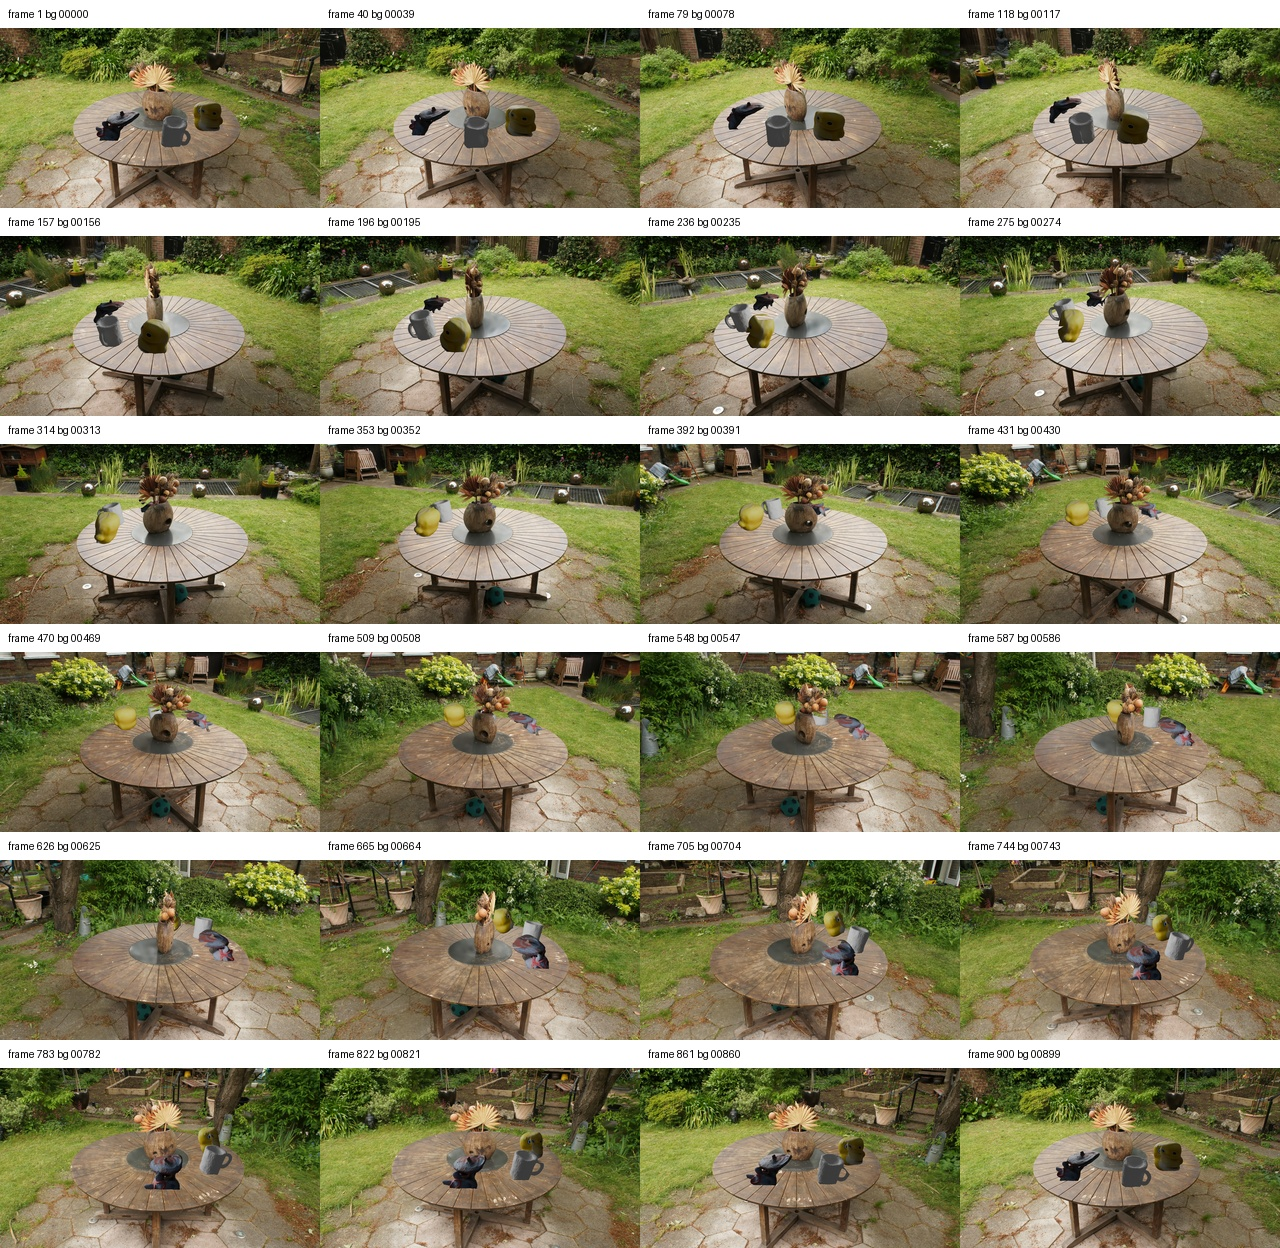
\includegraphics[width=0.66\textwidth]{reports/figures/final_scene_fusion_900f_1080p_contact.jpg}
\caption{Final Task 1 video contact sheet. The background is a 900-frame 2DGS trajectory, while A/B/C are rendered in Blender under the same camera JSON and composited with RGB/depth-aware masks.}
\label{fig:final_video_contact}
\vspace{3pt}
\captionof{table}{Comparison of the three Task 1 asset generation routes.}
\label{tab:method_compare}
\resizebox{0.98\textwidth}{!}{%
\begin{tabular}{p{2.1cm}p{2.4cm}p{2.5cm}p{3.1cm}p{3.1cm}p{3.4cm}}
\toprule
Route & Selected run & Compute time & Geometry evidence & Texture evidence & Main failure mode \\
\midrule
Multi-view A & Dense-half & COLMAP $<10$m; 2DGS $\sim$5m; eval $\sim$2m & 148/148 registered; 24125 COLMAP points; 2DGS PSNR 24.7654 & Real image colors remain in 2DGS renders; weak low-texture side blurs in mesh & TSDF export keeps table/background shells; component filtering cannot fully repair geometry \\
\midrule
Text-to-3D B & Style-constr. SDS & 10000 steps; 47:39 & 39314 vertices; 78628 faces; geometry score 4/5 & 1024$\times$1024 texture; texture score 3/5 & SDS hallucination, surface roughness, and possible Janus artifacts \\
\midrule
Single-image C & Magic123 mouse auto & Fine stage 17.18m & 23019 vertices; 46038 faces; front/oblique views usable & 2048$\times$2048 albedo; side/back texture smoothed & Original C rejected; mouse C still hallucinates hidden side/back geometry \\
\bottomrule
\end{tabular}
}
\end{figure*}

Figure~\ref{fig:final_video_contact} shows the final behavior across the full trajectory.
The camera moves around the garden table, the background lighting and viewpoint change continuously, and the three inserted objects remain in fixed tabletop positions.
The strongest frames show credible relative scale and partial occlusion with the real table centerpiece.
The weakest frames expose the remaining limitation: the compositor uses image-space depth rather than a physically unified 3D scene.
When the 2DGS depth around the vase, thin structures, or ambiguous foliage is unstable, the foreground mask can be partially overwritten by background texture.
This is documented as a limitation instead of being hidden, because it identifies the next technical step: true code-level insertion into a shared Gaussian or geometry representation.

\subsection{Comparison of the Three Generation Routes}
Table~\ref{tab:method_compare} summarizes the main comparison required by the assignment.
The conclusion is not that one route is universally better.
Multi-view reconstruction is the most physically grounded but is fragile when converted into a mesh.
Text-to-3D is the most flexible but has prior-driven geometry and texture.
Single-image-to-3D sits between the two: the visible input side is anchored, but hidden geometry is hallucinated.
For geometry accuracy, Object A is strongest before mesh export because it is constrained by registered cameras and real observations.
Object B is weaker geometrically because SDS optimizes toward a plausible prompt-conditioned object, not a measured target.
Object C is constrained in the input view but underconstrained elsewhere, so its side/back geometry is less reliable than its visible texture.
For texture detail, A again has the strongest evidence in image-space rendering, B has the weakest real-world grounding, and C preserves visible input-side appearance while hallucinating unseen texture.
For compute time, Magic123 is the cheapest among the final full generation runs, SDS is the most expensive, and Object A requires both CPU COLMAP and GPU 2DGS but remains efficient in the final dense-half run.
This comparison is the central empirical result of Task 1: the three pipelines can all contribute to the final scene, but their reliability is not equal.
Multi-view A is strongest before mesh export, text-generated B is usable after prompt filtering, and single-image C required rejecting the original object and replacing it with a simpler mouse input.
These differences also explain why the final fusion cannot use one universal coordinate correction for all objects.

\FloatBarrier

\section{Experiments: Task 2}
This section is reserved for Task 2.
\todo{Add Task 2 setup, main results, ablations, and discussion.}

\section{Conclusion}
Task 1 completes the required pipeline from background reconstruction to multi-source asset generation and synchronized video rendering.
The final solution is not a simple pasted image: it uses a 900-frame 2DGS camera trajectory and the same camera JSON for Blender foreground rendering.
The experiments also show why the final result still contains artifacts.
Object A is accurate through COLMAP and 2DGS but degrades during mesh extraction; Object B is prompt-flexible but SDS-prior driven; Object C exposes the strongest single-image ambiguity, requiring the original C to be rejected and a simpler mouse input to be used conservatively.
The final video is therefore a credible but imperfect fusion result, and its remaining errors are documented rather than hidden.
Task 2 will be added under the same report structure.

\appendix

\section*{Appendix}
\addcontentsline{toc}{section}{Appendix}

\section{Task 1 Experimental Details}

\subsection{Requirement Checklist and Artifact Map}
The Task 1 deliverables are mapped to concrete files in Table~\ref{tab:artifact_map}.
This table is intentionally explicit because the final submission must include not only the final video, but also intermediate evidence, scripts, configs, and links.

\begin{table*}[!t]
\centering
\caption{Task 1 artifact map. GitHub and ModelScope links are placeholders until final upload.}
\label{tab:artifact_map}
\scriptsize
\begin{tabular}{p{2.2cm}p{13.6cm}}
\toprule
Requirement & Evidence path \\
\midrule
Background & \figpath{background\_2dgs\_high}; \figpath{background\_2dgs\_metrics.csv} \\
Object A & \figpath{object\_a\_colmap\_dense}; \figpath{object\_a\_2dgs\_dense}; \figpath{object\_a\_stage\_evidence.jpg} \\
Object B & \figpath{text3d\_style\_constrained/model.obj}; \figpath{object\_b\_sds\_prompt\_ablation.csv} \\
Object C & \figpath{image3d\_mouse\_final\_clean/mesh.obj}; \figpath{object\_c\_old\_vs\_mouse\_reconstruction\_comparison.jpg} \\
Video & \figpath{final\_video\_900f\_1080p/final\_scene\_fusion\_15s\_60fps\_1080p.mp4} \\
Figures & \figpath{final\_scene\_fusion\_900f\_1080p\_contact.jpg}; \figpath{object\_a\_mouse\_background\_failure\_iterations.jpg} \\
GitHub / weights & [GitHub URL placeholder]; [ModelScope URL placeholder] \\
\bottomrule
\end{tabular}
\end{table*}

\begin{center}
\centering
\captionof{table}{A.1 background 2DGS configuration.}
\label{tab:app_bg_config}
\scriptsize
\begin{tabular}{lccc}
\toprule
Run & Iter. & Scene & Eval views \\
\midrule
Low & 5000 & garden & 24 \\
Mid & 15000 & garden & 24 \\
High & 30000 & garden & 24 \\
\bottomrule
\end{tabular}
\end{center}

\begin{center}
\centering
\captionof{table}{A.1 background 2DGS quantitative results.}
\label{tab:app_bg_result}
\scriptsize
\begin{tabular}{lccc}
\toprule
Run & PSNR$\uparrow$ & SSIM$\uparrow$ & LPIPS$\downarrow$ \\
\midrule
5k & 25.1907 & 0.7677 & 0.2556 \\
15k & 26.2062 & 0.8209 & 0.1812 \\
30k & \textbf{26.6501} & \textbf{0.8337} & \textbf{0.1638} \\
\bottomrule
\end{tabular}
\end{center}

\begin{center}
\centering
\captionof{table}{A.2 Object A frame extraction configuration.}
\label{tab:app_a_frames}
\scriptsize
\begin{tabular}{lccc}
\toprule
Set & FPS & Frames & Directory \\
\midrule
Sparse & 1 & 49 & \figpath{frames\_sparse} \\
Medium & 2 & 99 & \figpath{frames\_medium} \\
Dense & 3 & 148 & \figpath{frames\_dense} \\
\bottomrule
\end{tabular}
\end{center}

\subsection{Background 2DGS Ablation}
The background experiment is M1/R1 in the experiment matrix.
All three runs use the same Mip-NeRF 360 garden COLMAP scene, the same train/test split, and the same 2DGS code path.
Only the training iteration budget is changed.
This makes the ablation interpretable: any improvement is caused by optimization time rather than a different dataset, camera split, or renderer.
The concrete run configuration is shown in Table~\ref{tab:app_bg_config}.

Table~\ref{tab:app_bg_result} reports the measured results.
The low run trained for 5000 iterations and reached PSNR 25.1907.
The mid run trained for 15000 iterations and improved PSNR to 26.2062.
The high run trained for 30000 iterations and reached PSNR 26.6501.
The numerical gain from 15k to 30k is smaller than the gain from 5k to 15k, but it is still consistent across PSNR, SSIM, and LPIPS.
This is why the selected background is not chosen by a single metric.
The 30k model has the best perceptual score, LPIPS 0.1638, which matters for a moving garden video because vegetation, thin table boundaries, and specular clutter are visually amplified by camera motion.

The result pattern is expected for 2DGS optimization.
At 5k iterations, the model captures the coarse scene but still leaves high-frequency garden structures unstable.
At 15k, most camera-consistent structure is already fitted, so PSNR and SSIM jump.
At 30k, the remaining improvement is smaller because the easy low-frequency error has already been removed.
The useful gain is instead perceptual: the table boundary, foliage, and small background details become less noisy frame to frame.
For the final fusion, this is more important than raw training speed, because the three inserted objects are judged against the reconstructed table plane in every frame.

Figure~\ref{fig:bg_contact_appendix} shows the 24 test renders of the final background checkpoint.
These views also reveal why the final video uses a continuous 900-frame path instead of reusing the 24 test views: adjacent test views jump too much for a smooth video.
The final 900-frame trajectory was therefore rendered separately with \texttt{--render\_path\_frames 900}.

\begin{figure*}[t]
\centering
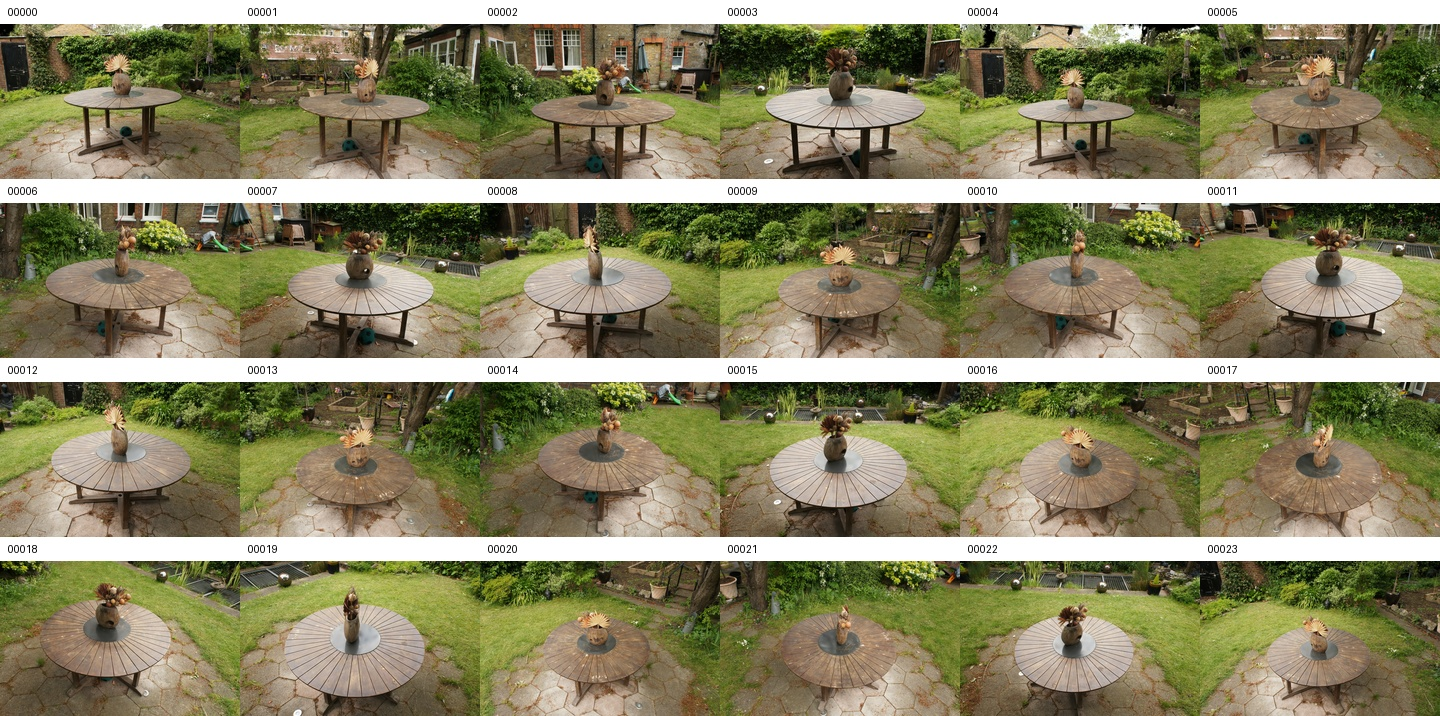
\includegraphics[width=0.98\linewidth]{reports/figures/background_2dgs_24_test_renders_contact.jpg}
\caption{The 24 held-out/test renders of the selected 30k garden 2DGS model. They are useful for evaluation and inspection, but too sparse for a smooth final video.}
\label{fig:bg_contact_appendix}
\end{figure*}

\subsection{Object A: Capture, COLMAP, 2DGS, and Mesh Export}
Object A required the most debugging because the real capture did not automatically become a clean mesh.
The experiment is split into four stages: video frame sampling, COLMAP registration, 2DGS training, and mesh export.
This separation is important.
The final visible artifact is not enough to say where the pipeline failed.
The evidence in Tables~\ref{tab:app_a_frames}--\ref{tab:app_a_stage} shows that the early reconstruction stages are mostly successful, while the neural-to-mesh conversion is the first stage that clearly damages the asset.

Table~\ref{tab:app_a_colmap} gives the COLMAP result.
Sparse sampling has the lowest reprojection error, 0.9727 px, but this does not make it the best source.
It registers only 35 images and creates only 4130 sparse points, so it has weak coverage of the object surface.
Medium sampling registers 87 images and 9837 points.
Dense sampling registers all 148 images, increases sparse points to 24125, and raises mean track length to 4.7546.
The reprojection error rises only slightly from medium to dense, 1.1265 px to 1.1296 px.
The interpretation is that dense sampling adds real correspondences rather than only noisy duplicates.
This is why the final Object A rerun uses the dense COLMAP model.

\begin{table}[t]
\centering
\caption{A.2 Object A COLMAP registration results.}
\label{tab:app_a_colmap}
\begin{tabular}{lrrrr}
\toprule
Set & Reg. & Points & Track & Reproj. \\
\midrule
Sparse & 35 & 4130 & 3.3637 & \textbf{0.9727} \\
Medium & 87 & 9837 & 4.1911 & 1.1265 \\
Dense & \textbf{148} & \textbf{24125} & \textbf{4.7546} & 1.1296 \\
\bottomrule
\end{tabular}
\end{table}

The 2DGS training configuration then compares medium-source full resolution, medium-source half resolution, and dense-source half resolution.
All three 2DGS runs use 15000 iterations.
The final dense-half run is not a weaker shortcut: it is a deliberate trade-off between camera coverage and image resolution.
Table~\ref{tab:app_a_2dgs} shows that dense-half reaches the best PSNR and LPIPS, 24.7654 and 0.3000, even though the full-resolution medium run has the highest SSIM.
The SSIM difference is not enough to override the PSNR/LPIPS and visual evidence because Object A has low-texture sides and thin geometry.
For this object, more registered viewpoints are more valuable than keeping the original resolution under weaker coverage.

\begin{table}[t]
\centering
\caption{A.2 Object A 2DGS configuration and results.}
\label{tab:app_a_2dgs}
\begin{tabular}{lrrrr}
\toprule
Run & Source & Res. & PSNR & LPIPS \\
\midrule
Full & Medium & 1 & 21.8139 & 0.3549 \\
Half & Medium & 2 & 22.4246 & 0.3245 \\
Dense-half & Dense & 2 & \textbf{24.7654} & \textbf{0.3000} \\
\bottomrule
\end{tabular}
\end{table}

Table~\ref{tab:app_a_stage} localizes the failure.
COLMAP dense reconstruction passes: 148/148 images are registered, with 24125 sparse points and mean reprojection error 1.1296 px.
2DGS image rendering also passes: the dense-half run reaches PSNR 24.7654, SSIM 0.8228, and LPIPS 0.3000 over 19 evaluation views.
The problem appears during mesh export.
The high-resolution TSDF export at mesh resolution 1024 contains 12.27M vertices and 23.78M faces, but much of that geometry is table/background shell.
Reducing mesh resolution to 256 makes the file manageable, 618102 vertices and 1171796 faces, but still keeps non-object geometry.
Connected-component filtering finally selects component\_02 with 19922 vertices and 38636 faces, which is usable for fusion but no longer as faithful as the original 2DGS image-space renderer.

\begin{table*}[t]
\centering
\caption{A.2 Object A stage-by-stage failure localization.}
\label{tab:app_a_stage}
\resizebox{0.98\textwidth}{!}{%
\begin{tabular}{p{3.0cm}p{4.1cm}p{4.6cm}p{4.2cm}}
\toprule
Stage & Artifact & Evidence & Interpretation \\
\midrule
COLMAP dense & \figpath{object\_a\_colmap\_dense} & 148/148 registered; 24125 points; 1.1296 px reprojection & Multiview registration is sufficient. \\
2DGS rendering & \figpath{object\_a\_2dgs\_dense} & PSNR 24.7654; SSIM 0.8228; LPIPS 0.3000 & Image-space color and view synthesis are acceptable. \\
Mesh export 1024 & \figpath{fuse\_post\_meshres1024.ply} & 12.27M vertices; 23.78M faces; 610.9 MB & Table/background shells dominate; not usable for fusion. \\
Mesh export 256 & \figpath{fuse\_post.ply} & 618102 vertices; 1171796 faces; 30.4 MB & Manageable but still contains non-object geometry. \\
Component filter & \figpath{component\_02.ply} & 19922 vertices; 38636 faces & Usable selected component, but incomplete surfaces remain. \\
\bottomrule
\end{tabular}
}
\end{table*}

\begin{table}[H]
\centering
\scriptsize
\caption{A.3 Object B SDS prompt configuration.}
\label{tab:app_b_config}
\resizebox{\linewidth}{!}{%
\begin{tabular}{p{1.6cm}p{4.5cm}p{1.0cm}p{1.1cm}p{1.1cm}}
\toprule
Variant & Prompt & Steps & Train res. & Batch size \\
\midrule
Simple & A clean ceramic mug & 10000 & 64$\times$64 & 1 \\
Detailed & A single matte ceramic mug with a simple handle, stable proportions, clean topology, neutral studio lighting & 10000 & 64$\times$64 & 1 \\
Style-constr. & A single realistic ceramic mug, no extra objects, no text, no face, neutral color, physically plausible shape & 10000 & 64$\times$64 & 1 \\
\bottomrule
\end{tabular}
}
\vspace{4pt}
\captionof{table}{A.3 Object B SDS prompt ablation results. Scores are on the fixed 1--5 rubric.}
\label{tab:app_b_result}
\resizebox{\linewidth}{!}{%
\begin{tabular}{p{1.4cm}p{1.0cm}rrrrrp{3.4cm}p{1.2cm}}
\toprule
Variant & Time & Vert. & Faces & Geo. & Tex. & Fusion & Artifact notes & Selection \\
\midrule
Simple & 49:41 & 33999 & 67786 & 3 & 3 & 3 & Recognizable mug and richer color, but fuzzy surface, ghosting, and unstable handle/body. & Rejected \\
Detailed & 50:03 & 3560 & 7060 & 2 & 2 & 2 & Blurrier geometry; default export failed and required threshold recovery; haze/background artifacts. & Rejected \\
Style-constr. & 47:39 & 39314 & 78628 & 4 & 3 & 4 & Cleanest silhouette and stable handle/body; neutral low-detail texture and minor roughness. & Selected \\
\bottomrule
\end{tabular}
}
\end{table}

This explains the apparently contradictory Object A observations.
In render/GT comparisons, Object A looks much better than in final fusion because 2DGS can render view-dependent appearance without committing to a watertight object mesh.
Blender fusion requires a mesh-like foreground asset, so the pipeline must export or filter geometry.
That step forces the splat representation into a surface representation and exposes table contamination, low-texture sides, and incomplete components.
Appendix C.1 gives the image evidence, including the later mouse control experiment that still fails because the capture is dominated by table/background pixels.

Per-view diagnostics give a more precise explanation.
The worst PSNR views include 00009=16.50, 00013=20.29, 00017=20.43, 00000=21.02, and 00012=22.43.
The best views include 00010=29.41, 00016=27.96, 00003=27.54, 00004=27.33, and 00007=27.33.
The umbrella-facing side has stronger color and silhouette cues.
The non-umbrella side is low-texture and close to table/background colors, so the mesh extraction step smears or removes it more easily.

\subsection{Object B: SDS Prompt Ablation}
Object B was generated by threestudio SDS with three prompt settings.
All three experiments use the same DreamFusion-style SDS configuration, 10000 optimization steps, 64$\times$64 training resolution, batch size 1, and the same Stable Diffusion checkpoint path.
The only intended variable is the text prompt.
Table~\ref{tab:app_b_config} records the concrete prompt configuration.

Table~\ref{tab:app_b_result} gives the export and scoring results.
The simple prompt produces a recognizable mug and richer color, but it also produces noisy/fuzzy surface structure, ghosting above the object, and less stable handle/body separation.
The detailed prompt is the surprising failure case.
It asks for clean topology and stable proportions, but the exported mesh has only 3560 vertices and 7060 faces, far smaller than the other two runs.
It also receives the lowest geometry, texture, and fusion-readiness scores.
The style-constrained prompt has the best geometry and fusion scores and is therefore selected.

The result is not a contradiction; it is a property of SDS optimization.
SDS does not reconstruct a measured object.
It optimizes a 3D representation so that rendered views receive favorable scores from a 2D diffusion prior.
A longer prompt can overconstrain the prior or create competing visual requirements.
In the detailed prompt, words such as ``matte,'' ``clean topology,'' and ``neutral studio lighting'' do not directly supervise a mesh topology loss.
They only bias the 2D prior, so the optimization can converge to a smoother, blurrier, lower-detail object that satisfies the prompt semantically but is less useful as a fused mesh.
The selected style-constrained prompt works better because it removes failure modes instead of adding decorative detail.
By saying no extra objects, no text, no face, and physically plausible shape, it reduces Janus-like ambiguity and keeps the object closer to a simple mug silhouette.
For final fusion, that stability matters more than a richer texture.

\subsection{Object C: Magic123 Mask Ablation}
Object C was tested with raw image, automatic background removal, and refined mask.
Raw input kept too much background appearance, causing texture contamination.
Refined mask looked cleaner as input, but the generated side geometry became more inflated and fragmented.
The auto-mask variant kept the clearest front-facing identity among the three, but final review rejected it as a successful 3D asset because side/back validation views were not stable.
This section records the ablation configuration and visual evidence; Appendix C explains the failure mechanism and the later mouse-C replacement.
The first-round evidence is kept in Appendix C, where it is discussed as a failure case rather than as a selected final asset.

\subsection{Fusion Layout, Pose, and Shadow Ablations}
Fusion was not a one-shot import.
The first garden composite, \texttt{fusion\_main\_layout\_v2}, made all three objects visible but placed them too large for the garden table.
Its scale/contact/lighting/viewpoint scores were 2/3/3/2 with four visible artifacts.
The next scale ablation used a global 0.78 scale.
It reduced the mismatch but still left A and C close to the table edge and allowed B to interfere with the vase.
The selected still-frame candidate, \texttt{fusion\_table\_insert\_v3}, used a tighter table footprint and a global 0.62 scale, improving the scores to 4/4/3/4 with two artifacts.
This early stage fixed the main spatial problem: the objects had to read as tabletop insertions rather than floating assets in the garden.

The later R6 ablation kept Object A's filtered \texttt{component\_02} and tested scale, position, and shadow controls.
The baseline v6 setting scored 3/3/4/3 for scale/contact/shadow/view stability.
The scale variant improved scale contact to 4 by reducing the visual dominance of A and C.
The position variant improved both scale and position contact to 4/4 because wider spacing avoided object overlap and gave the cleanest composition.
The no-shadow control was rejected: its shadow score dropped to 1, artifact count increased to 5, and the objects looked pasted onto the table.
This is the reason shadows are retained in the final scene even though the lighting is approximate.

Orientation was then handled separately in v7 because scale and contact scores can be good while the objects still face the wrong way.
The original v6 position run had good contact but Object A appeared inverted/ambiguous and Object B did not clearly show the mug handle.
Flipping A around the $y$ axis raised the A orientation score from 2 to 4.
Flipping B around $x$ or $y$ raised the mug orientation score from 1 to 4.
The selected still, \texttt{fusion\_table\_insert\_v7\_a\_flip\_y\_b\_flip\_x}, scored A orientation 4, B orientation 4, contact 4, and artifact count 3.
The remaining artifacts are therefore attributed less to pose and more to the imperfect A/C meshes.
Figure~\ref{fig:fusion_ablation_appendix} shows the scale/position/shadow evidence, and Fig.~\ref{fig:fusion_orientation_appendix} shows the orientation evidence.

\begin{figure*}[!tbp]
\centering
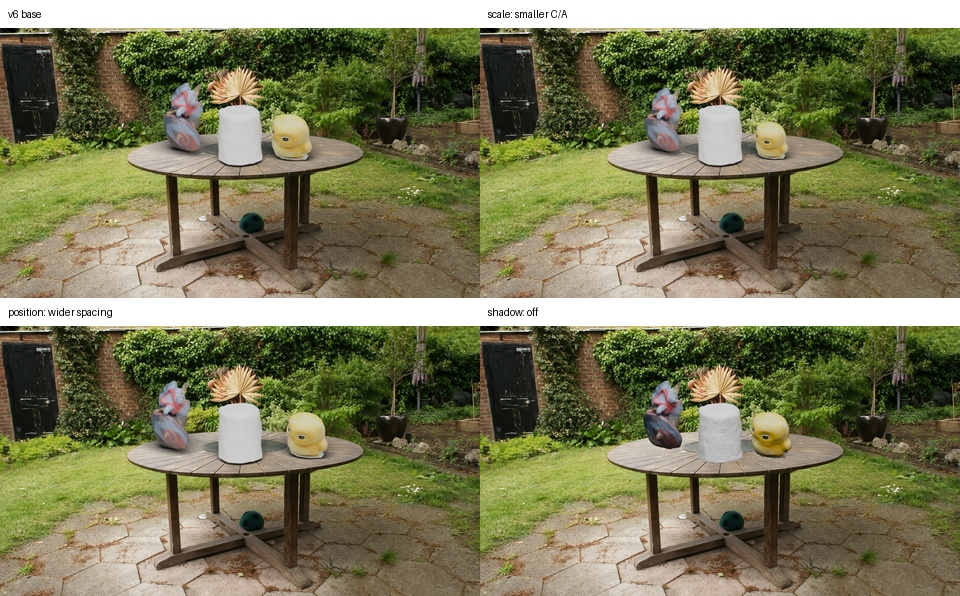
\includegraphics[width=\textwidth,height=0.34\textheight,keepaspectratio]{reports/figures/fusion_v6_ablation_contact.jpg}
\caption{Fusion v6 scale/position/shadow ablation. The selected variant improves spacing and contact while keeping shadows.}
\label{fig:fusion_ablation_appendix}
\end{figure*}

\begin{figure*}[!tbp]
\centering
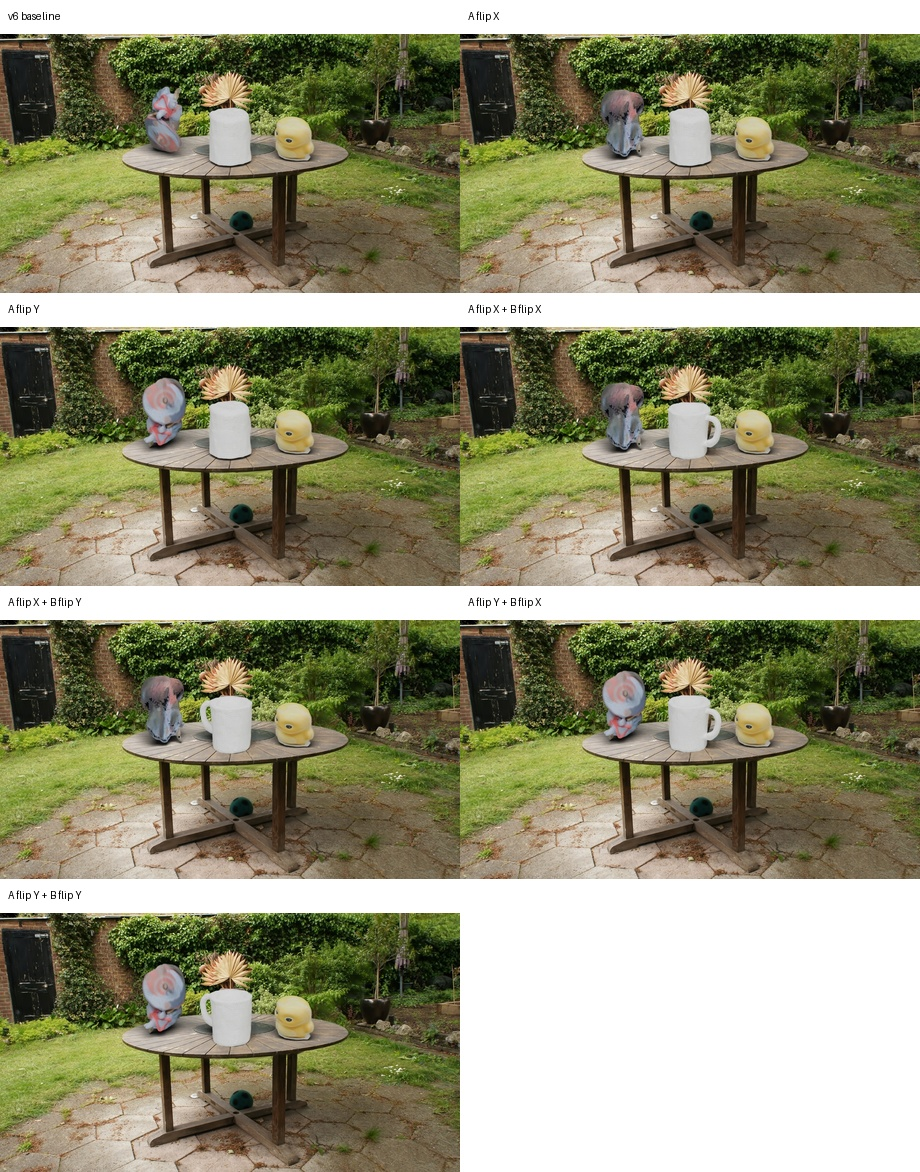
\includegraphics[width=\textwidth,height=0.34\textheight,keepaspectratio]{reports/figures/fusion_v7_orientation_contact.jpg}
\caption{Fusion v7 orientation ablation. A/B rotations are adjusted before the synchronized final video.}
\label{fig:fusion_orientation_appendix}
\end{figure*}

The final frozen pose uses the following pre-freeze tuning values:
A=(610,480), B=(815,500), C=(990,480) as placement pixels;
A=1.55, B=1.20, C=1.70 as scale multipliers;
A=(-30,90,0), B=(130,10,0), C=(90,-20,20) as rotation deltas;
and A=-0.65, B=-0.60, C=-0.60 as height offsets.
After freezing into the scene file, the final transform parameters are those reported in Table~\ref{tab:frozen_pose}.
These parameters were found by enumeration rather than by solving a single linear alignment.
The reason is practical: A, B, and C come from different generators and their local axes are not semantically consistent.
Object A is a filtered component from a 2DGS mesh export, Object B is a generated SDS mesh with arbitrary canonical orientation, and Object C is inferred from one image.
Without reliable 3D correspondences between each object coordinate frame and the garden 2DGS frame, a single closed-form transform would look more rigorous than it actually is.
The constrained search records the actual decision process: keep the objects on the table, preserve readable orientation, retain contact shadow, and avoid hiding the garden centerpiece.

\subsection{Final Video Rendering Configuration}
The final video has 900 composite frames.
The background renderer command uses the selected garden 30k checkpoint and exports \texttt{cameras\_900.json}.
The synchronized compositor then runs Blender with 16 samples at 1920$\times$1080 and 60 fps.
The final output is stored at \figpath{runs/scene/final_video_900f_1080p/final_scene_fusion_15s_60fps_1080p.mp4}.
The file was verified with \texttt{ffprobe}: width 1920, height 1080, frame rate 60/1, 900 frames, duration 15.0 seconds, and size 19500904 bytes.
The 900-frame setting is not arbitrary.
The final video targets 60 fps and 15 seconds, so 900 frames gives a smooth path while preserving enough duration to show the background first, approach the table, orbit the inserted objects, and end with a wider view.
The 24 held-out garden views are useful for metric evaluation, but they are too sparse for this motion; direct interpolation over a 900-frame path avoids visible camera jumps.

The rendering pipeline has two synchronized outputs per frame.
First, the garden 2DGS checkpoint renders RGB and depth along the final camera path.
Second, Blender renders A/B/C with the same camera intrinsics and extrinsics from \texttt{cameras\_900.json}.
The foreground render uses transparent RGBA output and 16 samples, which is a compromise between clean edges and reasonable render time.
The compositor then combines foreground and background using RGB/depth-aware masks.
This makes the objects fixed in world position while the viewer moves around them.
It also explains the remaining failure mode: if the 2DGS background depth is wrong near thin structures such as the vase or foliage, the image-space depth comparison can partially overwrite a foreground object.

The final video is therefore evaluated as a synchronized multi-view artifact, not a single still.
The expected success condition is that A/B/C stay fixed on the same tabletop locations across camera motion, that their relative scale remains plausible, and that shadows or contact cues prevent them from reading as flat pasted sprites.
The expected limitation is that the garden and the inserted meshes are still not one physical 3D representation.
The background is a 2DGS render, while A/B/C are mesh foreground renders composited afterward.
This is why the report keeps the fusion errors visible and treats Gaussian-level insertion as a future extension rather than claiming a perfect shared-scene reconstruction.

\FloatBarrier

\section{Task 1 Mathematical Formulation}

\subsection{Camera Projection Model}
Let a garden world point be $X_w\in\mathbb{R}^3$ and its homogeneous form be $\tilde X_w=[X_w^\top,1]^\top$.
For intrinsic matrix
\[
K=\begin{bmatrix} f_x&0&c_x\\0&f_y&c_y\\0&0&1\end{bmatrix},
\]
rotation $R$, and camera center $C$, the camera coordinate is
\[
X_c=R^\top(X_w-C)=\begin{bmatrix}x_c\\y_c\\z_c\end{bmatrix}.
\]
Equivalently, the full projective camera is
\[
\lambda
\begin{bmatrix}u\\v\\1\end{bmatrix}
=
P\tilde X_w,\qquad
P=K\begin{bmatrix}R^\top&-R^\top C\end{bmatrix},
\]
where $\lambda=z_c$ for the pinhole model and a point is visible only when $z_c>0$.
The projected pixel is
\[
u=f_x\frac{x_c}{z_c}+c_x,\qquad
v=f_y\frac{y_c}{z_c}+c_y.
\]
This perspective division is the only nonlinear part of the projection.
Its Jacobian with respect to the camera-space point is
\[
J_{\pi,c}
=
\frac{\partial(u,v)}{\partial(x_c,y_c,z_c)}
=
\begin{bmatrix}
f_x/z_c & 0 & -f_xx_c/z_c^2\\
0 & f_y/z_c & -f_yy_c/z_c^2
\end{bmatrix}.
\]
Since $X_c=R^\top(X_w-C)$, the world-space projection Jacobian is
\[
J_{\pi,w}=J_{\pi,c}R^\top .
\]
For a small 3D placement error $\delta X_w$, the induced image displacement is therefore
\[
\delta p \approx J_{\pi,w}\delta X_w,\qquad
\|\delta p\|_2\le \|J_{\pi,w}\|_2\|\delta X_w\|_2 .
\]
The bound shows why foreground placement becomes visually fragile for close cameras or shallow depths: the terms $1/z_c$ and $1/z_c^2$ amplify small 3D errors into pixel-level misalignment.

The final video uses the same $K$, $R$, and $C$ sequence for 2DGS background rendering and Blender foreground rendering.
Let $\pi_{\mathrm{bg}}$ and $\pi_{\mathrm{fg}}$ denote the two renderers' projection functions.
Synchronization means
\[
\pi_{\mathrm{bg}}(X_w;K,R,C)=\pi_{\mathrm{fg}}(X_w;K,R,C)
\]
for the shared camera path.
If Blender used perturbed parameters $(K+\delta K,R\exp([\delta\omega]_\times),C+\delta C)$, the first-order reprojection drift would be
\[
\delta p
\approx
J_K\delta K
+J_R\delta\omega
+J_C\delta C,
\]
which would make A/B/C slide relative to the garden even if the meshes were static in 3D.
This is the mathematical reason the final video is synchronized rather than a moving backplate with independently moving objects.

\subsection{Depth-based Pixel-to-World Placement}
Given a 2DGS depth value $d$ at pixel $(u,v)$, the camera-space point is
\[
X_c=dK^{-1}\begin{bmatrix}u\\v\\1\end{bmatrix}
=
\begin{bmatrix}
d(u-c_x)/f_x\\
d(v-c_y)/f_y\\
d
\end{bmatrix}.
\]
The world-space point is
\[
X_w=RX_c+C.
\]
This is used for the coarse placement of A/B/C on the garden table.

Let the pixel/depth perturbation be $(\delta u,\delta v,\delta d)$.
The first-order perturbation is
\[
\delta X_c=
\frac{\partial X_c}{\partial u}\delta u+
\frac{\partial X_c}{\partial v}\delta v+
\frac{\partial X_c}{\partial d}\delta d,
\]
where
\[
\begin{aligned}
\frac{\partial X_c}{\partial u}&=
\begin{bmatrix}d/f_x\\0\\0\end{bmatrix},&
\frac{\partial X_c}{\partial v}&=
\begin{bmatrix}0\\d/f_y\\0\end{bmatrix},\\
\frac{\partial X_c}{\partial d}&=
\begin{bmatrix}(u-c_x)/f_x\\(v-c_y)/f_y\\1\end{bmatrix}.
\end{aligned}
\]
Since $\delta X_w=R\delta X_c$ and $R$ is orthonormal,
\[
\|\delta X_w\|
\le
\left\|\frac{\partial X_c}{\partial u}\right\||\delta u|
+
\left\|\frac{\partial X_c}{\partial v}\right\||\delta v|
+
\left\|\frac{\partial X_c}{\partial d}\right\||\delta d|.
\]
Depth placement is therefore sensitive to depth noise and pixel choice, especially when the chosen point lies on a table edge, vase boundary, or thin structure.
This bound justifies the later height and contact enumeration.

\subsection{Mesh Coordinate Transform and Perturbation}
Let an asset vertex be $\tilde X_a=[X_a^\top,1]^\top$.
The transform used by the Blender insertion can be written as a homogeneous matrix chain
\[
\begin{aligned}
\tilde X_f
&=H(\phi)\tilde X_a\\
&=
T_{\mathrm{loc}}
T_{\mathrm{contact}}
R_z(\theta_z)R_y(\theta_y)R_x(\theta_x)\\
&\quad
S(s)T_{\mathrm{center}}A_{\mathrm{up}}\tilde X_a .
\end{aligned}
\]
where $\phi=(s,\theta_x,\theta_y,\theta_z,t)$ is the tunable pose.
$A_{\mathrm{up}}$ converts the source up-axis convention, $T_{\mathrm{center}}$ recenters the asset by its mesh bounding box or centroid, $S(s)=\mathrm{diag}(s,s,s,1)$ gives an isotropic scale, the Euler rotations choose the visible canonical side, $T_{\mathrm{contact}}$ enforces table contact, and $T_{\mathrm{loc}}$ moves the object to the selected garden location.
After centering and up-axis conversion, let $X=T_{\mathrm{center}}A_{\mathrm{up}}X_a$ and combine the final translations into $t$.
The Euclidean part is then
\[
X_f=sR(\theta)X+t .
\]

For a small perturbation $\delta\phi=(\delta s,\delta\omega,\delta t)$ around a chosen pose, using the Lie algebra approximation
\[
R(\theta+\delta\omega)\approx R(\theta)(I+[\delta\omega]_\times),
\]
the first-order vertex perturbation is
\[
\delta X_f
\approx
R X\,\delta s
-sR[X]_\times\delta\omega
+\delta t .
\]
Therefore
\[
\|\delta X_f\|_2
\le
\|X\|_2|\delta s|
+s\|X\|_2\|\delta\omega\|_2
+\|\delta t\|_2 .
\]
This inequality is important for the real fusion results.
Large or off-center meshes amplify rotation error, so a mug handle, an umbrella-like structure, or an incomplete shell can move visibly even when the numerical angle change is small.
Scale error is also not uniform perceptually: a small $\delta s$ is most visible at the asset silhouette and at the contact boundary because those regions define the perceived object size.

The contact translation can be expressed with a table plane.
Let the local table plane be
\[
\Pi=\{X:n^\top X+b=0\},\qquad \|n\|_2=1 ,
\]
where $n$ is the table normal estimated from the selected garden view/depth.
For a transformed mesh with vertices $Y_i=sRX_i+t_{\mathrm{loc}}$, the lowest signed distance is
\[
m(\phi)=\min_i(n^\top Y_i+b).
\]
The ideal hard-contact correction is
\[
t_{\mathrm{contact}}=-m(\phi)n .
\]
If $m(\phi)>0$, the object floats above the table; if $m(\phi)<0$, it penetrates the table.
Under a perturbation, the signed contact error changes as
\[
\delta m
\approx
n^\top(RX_{i^\star}\delta s-sR[X_{i^\star}]_\times\delta\omega+\delta t),
\]
where $i^\star$ is the vertex that attains the minimum distance.
This explains a practical observation from the fusion search: scale, rotation, and height cannot be tuned independently.
Changing rotation changes which vertex becomes the lowest point; changing scale changes the signed table distance; changing height fixes contact in one view but may expose penetration from another view.

The final pose selection can be viewed as a constrained optimization problem rather than an arbitrary manual adjustment.
For each asset $k\in\{A,B,C\}$ and candidate pose $\phi_k$, the search minimizes an image-space and contact-space objective
\[
\begin{aligned}
\mathcal{E}(\phi_k)
&=
w_c|m(\phi_k)|
+w_p\|\pi(X_f(\phi_k))-p_k^\star\|_2\\
&\quad
+w_oE_{\mathrm{orient}}(\phi_k)
+w_vE_{\mathrm{view}}(\phi_k).
\end{aligned}
\]
where $p_k^\star$ is the desired tabletop image location, $E_{\mathrm{orient}}$ penalizes a semantically wrong visible side, and $E_{\mathrm{view}}$ penalizes instability across the camera path.
In the implementation these terms were not optimized by gradients because the required signals are not fully differentiable: orientation is judged semantically, contact depends on incomplete mesh geometry, and the 2DGS background provides imperfect depth around thin objects.
The discrete search over scale, rotation, and height is therefore the practical approximation to the objective above.

This mathematical form maps directly to the observed failures.
Object A has a real multi-view origin, but the exported mesh still contains incomplete shells and weak texture on some sides; its $X_i$ distribution and visible silhouette are therefore unreliable for some rotations.
Object B has a cleaner generated mesh but an arbitrary canonical frame, so $A_{\mathrm{up}}$ and $R(\theta)$ are semantic choices rather than measured calibration.
Object C is inferred from one image, so the back and side geometry are hallucinated; the contact vertex $i^\star$ can be geometrically plausible in one view and wrong in another.
This is why the final system records the chosen scale, rotation, and height instead of claiming a universal object-to-garden linear transform.

\subsection{Why a Single Linear Alignment Was Not Used}
A natural question is why the three assets were not inserted by estimating one closed-form similarity transform from object coordinates to garden coordinates.
Mathematically, that would require paired 3D correspondences
\[
\mathcal{C}=\{(X_a^i,X_g^i)\}_{i=1}^N,
\]
where $X_a^i$ is a point on the asset and $X_g^i$ is the same physical point expressed in the garden frame.
If such pairs existed, the optimal isotropic similarity transform could be written as
\[
\min_{s,R,t}\sum_i\|X_g^i-(sRX_a^i+t)\|_2^2,
\quad R^\top R=I,\ \det(R)=1.
\]
With centered points $\bar X_a^i=X_a^i-\mu_a$ and $\bar X_g^i=X_g^i-\mu_g$,
\[
\Sigma=\frac{1}{N}\sum_i \bar X_g^i(\bar X_a^i)^\top,\qquad
\Sigma=UDV^\top .
\]
The Procrustes/Umeyama solution is
\[
\begin{aligned}
R&=USV^\top,\\
s&=\frac{\mathrm{tr}(DS)}{\sigma_a^2},\\
t&=\mu_g-sR\mu_a,
\end{aligned}
\]
where $S=\mathrm{diag}(1,1,\det(UV^\top))$ prevents reflection and $\sigma_a^2=N^{-1}\sum_i\|\bar X_a^i\|_2^2$.
This solution is rigorous, but only under a strong assumption: the two point sets must describe the same object geometry with reliable point-to-point matches.

That assumption is false for the present fusion task.
The garden scene contains a table and background, but it does not contain the three inserted objects before fusion.
Thus there is no real $X_g^i$ corresponding to a mug handle, an umbrella surface, or the single-image object back side.
At most we have weak constraints: a desired image-space location, a table contact plane, and a semantic orientation such as ``show the handle'' or ``keep the better side visible.''
These constraints are lower-dimensional and partly semantic; they do not define a full set of 3D correspondences.

Even if pseudo-correspondences were manually chosen, the estimator would be biased by reconstruction artifacts.
Suppose the observed target relation were
\[
X_g^i=s_0R_0X_a^i+t_0+\epsilon_i,
\]
where $\epsilon_i$ is not zero-mean noise but systematic error from shell fragments, missing texture, hallucinated side geometry, or unstable depth.
Then the empirical covariance becomes
\[
\Sigma
=
s_0R_0\Sigma_a
+
\frac{1}{N}\sum_i(\epsilon_i-\bar\epsilon)(\bar X_a^i)^\top .
\]
The second term rotates and scales the SVD solution away from the true pose.
Therefore the closed-form solution would not merely be noisy; it would fit the artifacts as if they were valid geometry.
This is especially harmful for Object A, whose exported mesh keeps useful color on one side but still has incomplete components, and for Object C, whose side/back geometry is inferred rather than measured.

An ICP-style variant would not solve the issue either.
Point-to-surface registration would minimize a distance such as
\[
\min_{s,R,t}\sum_i
\rho\!\left(
d_{\mathcal{S}_g}(sRX_a^i+t)
\right),
\]
where $d_{\mathcal{S}_g}$ is distance to the garden surface and $\rho$ is a robust penalty.
But the correct target is not to make the asset mesh lie on the garden surface; only the contact region should touch the table, while the rest of the object should remain above it.
Optimizing all vertices against the garden surface would collapse the object into the table or align it with unrelated background geometry.

The actual method therefore uses a constrained search rather than a single linear alignment.
Depth unprojection provides a coarse table anchor, the contact-plane formula controls height, and the discrete pose grid searches over scale and rotations that preserve semantic visibility.
This is less elegant than Umeyama alignment, but it matches the available evidence.
The final recorded transform is consequently an experimentally selected pose under partial constraints, not a solved object-to-object registration.

\subsection{Depth-aware Alpha Compositing}
Let the image domain be $\Omega=\{1,\ldots,W\}\times\{1,\ldots,H\}$.
For a pixel $p=(u,v)\in\Omega$, Blender produces foreground RGB, alpha, and depth
\[
(I_f(p),\alpha_f(p),D_f(p)),
\]
where $I_f(p)\in[0,1]^3$, $\alpha_f(p)\in[0,1]$, and $D_f(p)$ is the foreground camera depth.
The 2DGS renderer produces background RGB and depth
\[
(I_b(p),D_b(p)).
\]
Before comparison, $D_f$ and $D_b$ are converted to the same camera-depth convention, with smaller depth meaning closer to the camera.
The alpha threshold $\tau_\alpha$ removes transparent foreground pixels, while the depth tolerance $\tau_d$ absorbs small calibration and reconstruction errors.
In the final video $\tau_d=0.08$ in the normalized depth scale used by the compositor.

Naive alpha compositing ignores depth and blends every foreground pixel with nonzero alpha:
\[
I_{\mathrm{naive}}(p)
=
\alpha_f(p)I_f(p)+(1-\alpha_f(p))I_b(p).
\]
This works only when the foreground object should always appear in front of the background.
It fails in a reconstructed scene because some background structures may be physically closer than the inserted mesh along a particular camera ray.
The depth-aware visibility mask is therefore
\[
M_f(p)=
\mathbb{1}\left[
\alpha_f(p)>\tau_\alpha
\land
D_f(p)<D_b(p)+\tau_d
\right].
\]
First define the alpha-blended foreground candidate
\[
C_f(p)
=
\alpha_f(p)I_f(p)+(1-\alpha_f(p))I_b(p).
\]
The final composite is
\[
I(p)=M_f(p)C_f(p)+(1-M_f(p))I_b(p).
\]
Thus $M_f(p)=1$ means the foreground is allowed to contribute at pixel $p$; $M_f(p)=0$ means the background overwrites it.

The decision boundary is easier to analyze through the signed depth margin
\[
g(p)=D_b(p)-D_f(p)+\tau_d .
\]
Ignoring alpha for the moment, the foreground is visible when $g(p)>0$.
Let the true depths be $D_f^\star,D_b^\star$ and the measured depths be
\[
D_f=D_f^\star+\epsilon_f,\qquad
D_b=D_b^\star+\epsilon_b .
\]
The measured margin is
\[
g=g^\star+\epsilon_b-\epsilon_f,
\quad
g^\star=D_b^\star-D_f^\star+\tau_d .
\]
A foreground/background visibility flip can occur when the perturbation changes the sign of the margin:
\[
|g^\star(p)|
\le
|\epsilon_f(p)|+|\epsilon_b(p)|.
\]
Equivalently, pixels near the depth boundary are unstable even if the RGB render looks plausible.
This is the formal reason that a single good still frame does not guarantee a stable video composite.

Alpha uncertainty gives a second failure mode.
Let the foreground matte have error $\epsilon_\alpha$ so that $\alpha_f=\alpha_f^\star+\epsilon_\alpha$.
Near object boundaries, a matte flip can occur when
\[
|\alpha_f^\star(p)-\tau_\alpha|\le |\epsilon_\alpha(p)|.
\]
Depth and alpha errors are coupled in practice: boundary pixels of A/B/C often have partial transparency, anti-aliased edges, or imperfect mesh silhouettes, exactly where depth comparison is also least reliable.
The observed false occlusions around the table centerpiece and thin garden structures are therefore expected.
Those pixels have small $|g^\star|$ because the foreground and background depths are close, and the 2DGS depth is less stable around thin objects.
The tolerance $\tau_d$ reduces flicker but cannot remove all errors: increasing it keeps more foreground but risks drawing objects through real foreground background structures; decreasing it respects background depth but can cut holes into A/B/C.

\subsection{Metrics and Discrete Rubric}
For image-based reconstruction metrics,
\[
\begin{aligned}
\mathrm{MSE}
&=\frac{1}{HW}\sum_{u,v}\|I(u,v)-\hat I(u,v)\|^2,\\
\mathrm{PSNR}
&=10\log_{10}\frac{I_{\max}^2}{\mathrm{MSE}}.
\end{aligned}
\]
SSIM is
\[
\mathrm{SSIM}(x,y)=
\frac{(2\mu_x\mu_y+C_1)(2\sigma_{xy}+C_2)}
{(\mu_x^2+\mu_y^2+C_1)(\sigma_x^2+\sigma_y^2+C_2)}.
\]
LPIPS is treated as a learned feature distance,
\[
\mathrm{LPIPS}(x,y)=\sum_l w_l\|\phi_l(x)-\phi_l(y)\|_2^2.
\]
For B/C, there are no held-out ground-truth views.
Their selection therefore uses a discrete objective
\[
Q=w_g q_{\mathrm{geometry}}+w_t q_{\mathrm{texture}}+w_f q_{\mathrm{fusion}}-w_a n_{\mathrm{artifact}},
\]
where each $q$ is scored from 1 to 5 with a fixed rubric.
This is not a replacement for ground-truth metrics; it is a controlled selection rule for generated assets without multi-view supervision.

\section{Task 1 Detailed Analysis and Failure Cases}

\subsection{Object A Failure Localization}
The strongest evidence for Object A is that failure is stage-dependent rather than a uniform failure of the whole multi-view pipeline.
COLMAP registers the dense run successfully, with 148/148 registered images, 24125 sparse points, and 1.1296 px mean reprojection error.
The dense-half 2DGS run is also quantitatively usable, with PSNR 24.7654, SSIM 0.8228, and LPIPS 0.3000 over 19 evaluation views.
These numbers do not mean the object is perfect, but they localize the first hard failure after image-space rendering.
The visible degradation begins when the 2DGS representation is forced into a mesh for Blender fusion.

The cause is the capture distribution.
Object A occupies only part of the phone frames, while the table and nearby background occupy a large, static region.
COLMAP and 2DGS therefore receive many confident observations of non-object surfaces.
In image-space novel-view rendering this is tolerable because 2DGS can render the complete local scene around the object.
For insertion, however, the assignment needs a separable asset.
The mesh\_res=1024 export has 12.27M vertices, 23.78M faces, and 610.9 MB size, but much of that geometry is table/background shell rather than Object A.
The mesh\_res=256 output is smaller, with 618102 vertices, 1171796 faces, and 30.4 MB size, but it still keeps non-object geometry.
Connected-component filtering selects component\_02 with 19922 vertices and 38636 faces, removing most table shell but not restoring missing object surfaces.

To test whether this was only caused by the original object's shape complexity, a simpler mouse was reconstructed as an additional Object A control.
This control has an easier silhouette and smoother surface than the original object, so a clean result would have supported the hypothesis that the old object itself was too complex.
The result does not support that hypothesis.
The mouse image-space 2DGS render remains visually close to the held-out frames, but the separable foreground asset still fails after export and filtering.
The input views contain a large white desk, floor, chair legs, and other static background surfaces; those regions occupy much more image area than the mouse and are observed consistently across frames.
Consequently, the optimized 2DGS field models the mouse and the surrounding desk/background together.

Figure~\ref{fig:a_mouse_background_iterations} shows the failed optimization sequence.
The first row shows the data and stage transition: the mouse is small in the captured frames, 2DGS render/GT pairs remain plausible, but TSDF/component export contains desk and background structures.
The second row shows three Gaussian proxy attempts.
The initial proxy crop keeps 4850 of 113502 Gaussians but still contains table shell.
The tighter crop reduces this to 2677 Gaussians, but it removes useful mouse structure before removing all background.
Relaxing the opacity threshold recovers 4392 Gaussians and a more solid proxy, but it also brings back background points.
This repeated failure is why the report attributes Object A's final degradation primarily to background-dominated object separation rather than to a lack of training iterations.

\begin{figure*}[!tbp]
\centering
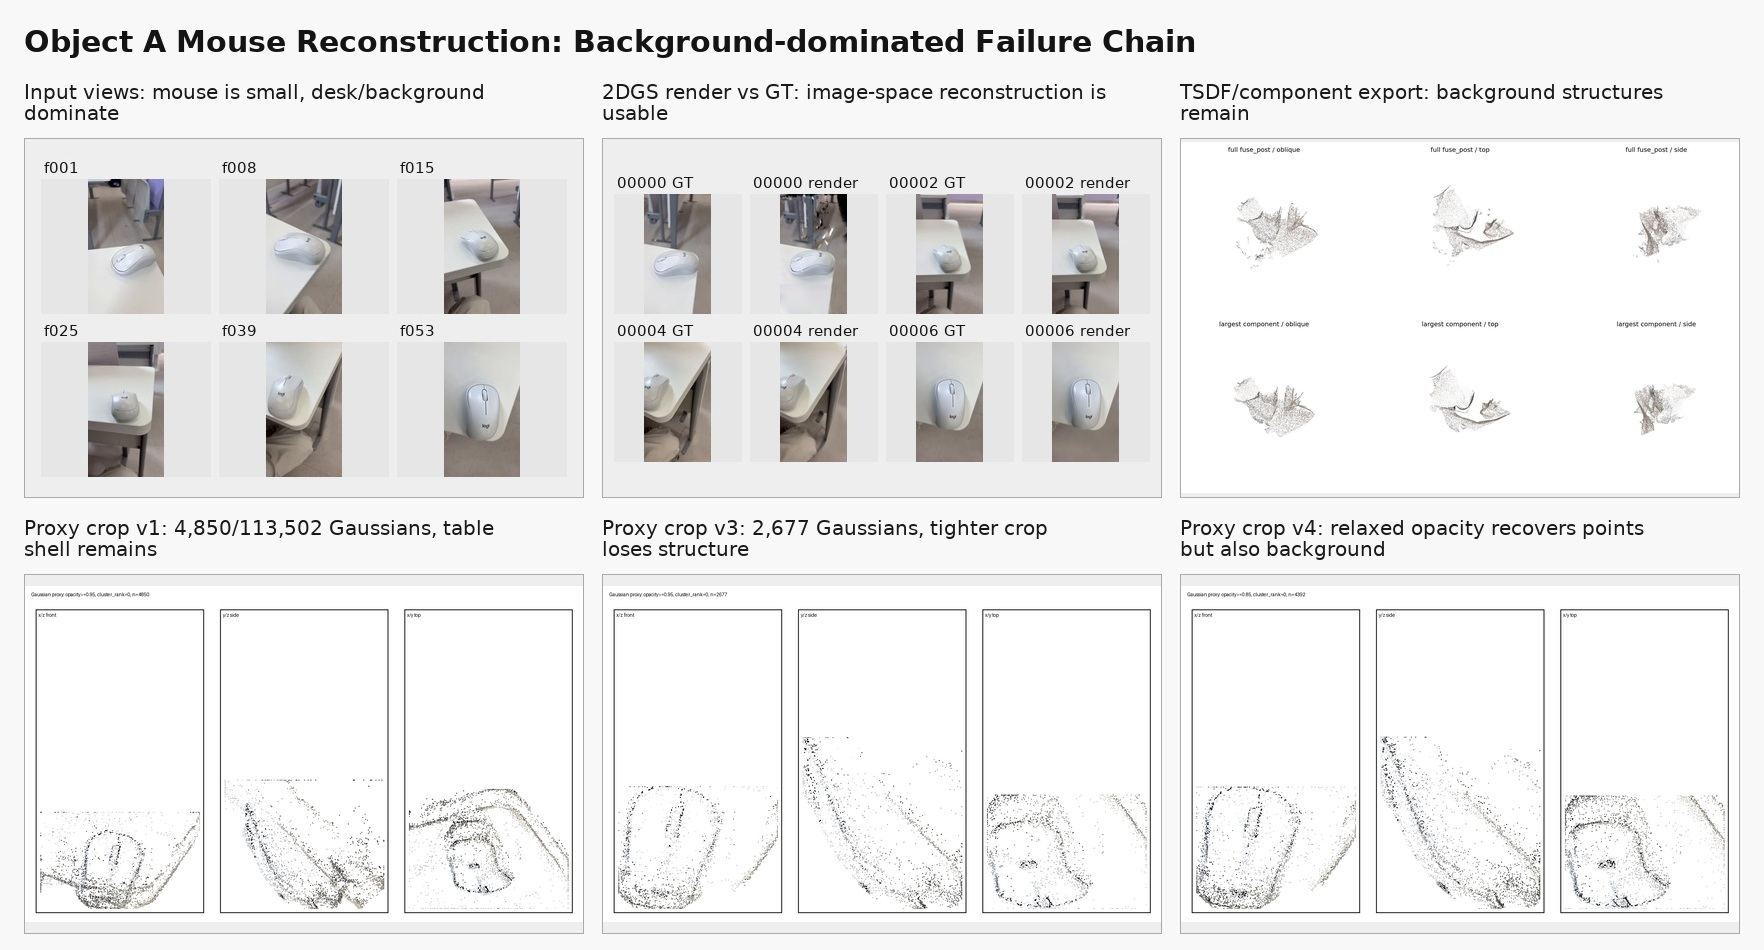
\includegraphics[width=\textwidth,height=0.42\textheight,keepaspectratio]{reports/figures/object_a_mouse_background_failure_iterations.jpg}
\caption{Mouse control experiment for Object A failure localization. A simpler mouse improves image-space recognition, but repeated mesh/proxy extraction still mixes the object with desk and background geometry. The experiment supports the diagnosis that Object A's fusion failure is driven by background-dominated capture and object/background separation, not only by the original object's complexity.}
\label{fig:a_mouse_background_iterations}
\end{figure*}

This chain explains the visual symptoms.
The umbrella-facing side remains recognizable because it has stronger color contrast and a distinctive silhouette.
The opposite side is blurrier because it has lower texture, weaker silhouette cues, and colors closer to the table/background distribution.
When the current Blender rerender path is applied to the old A asset, the color can regress from the accepted red/blue foreground to a gray/white appearance.
The crop measurement is concrete: for background frame 00000, the old final A crop has mean RGB [149.27, 137.80, 125.87], while the rerendered A crop has [85.96, 80.75, 74.61]; for frame 00156, the old crop has [198.48, 189.63, 159.86], while the rerendered crop has [83.98, 77.52, 68.66].
Figure~\ref{fig:a_color_regression_appendix} shows this regression.
This is why the final replacement-C video preserves the old accepted A/B foreground instead of rerendering A through the current mesh/material path.

\begin{figure*}[!tbp]
\centering
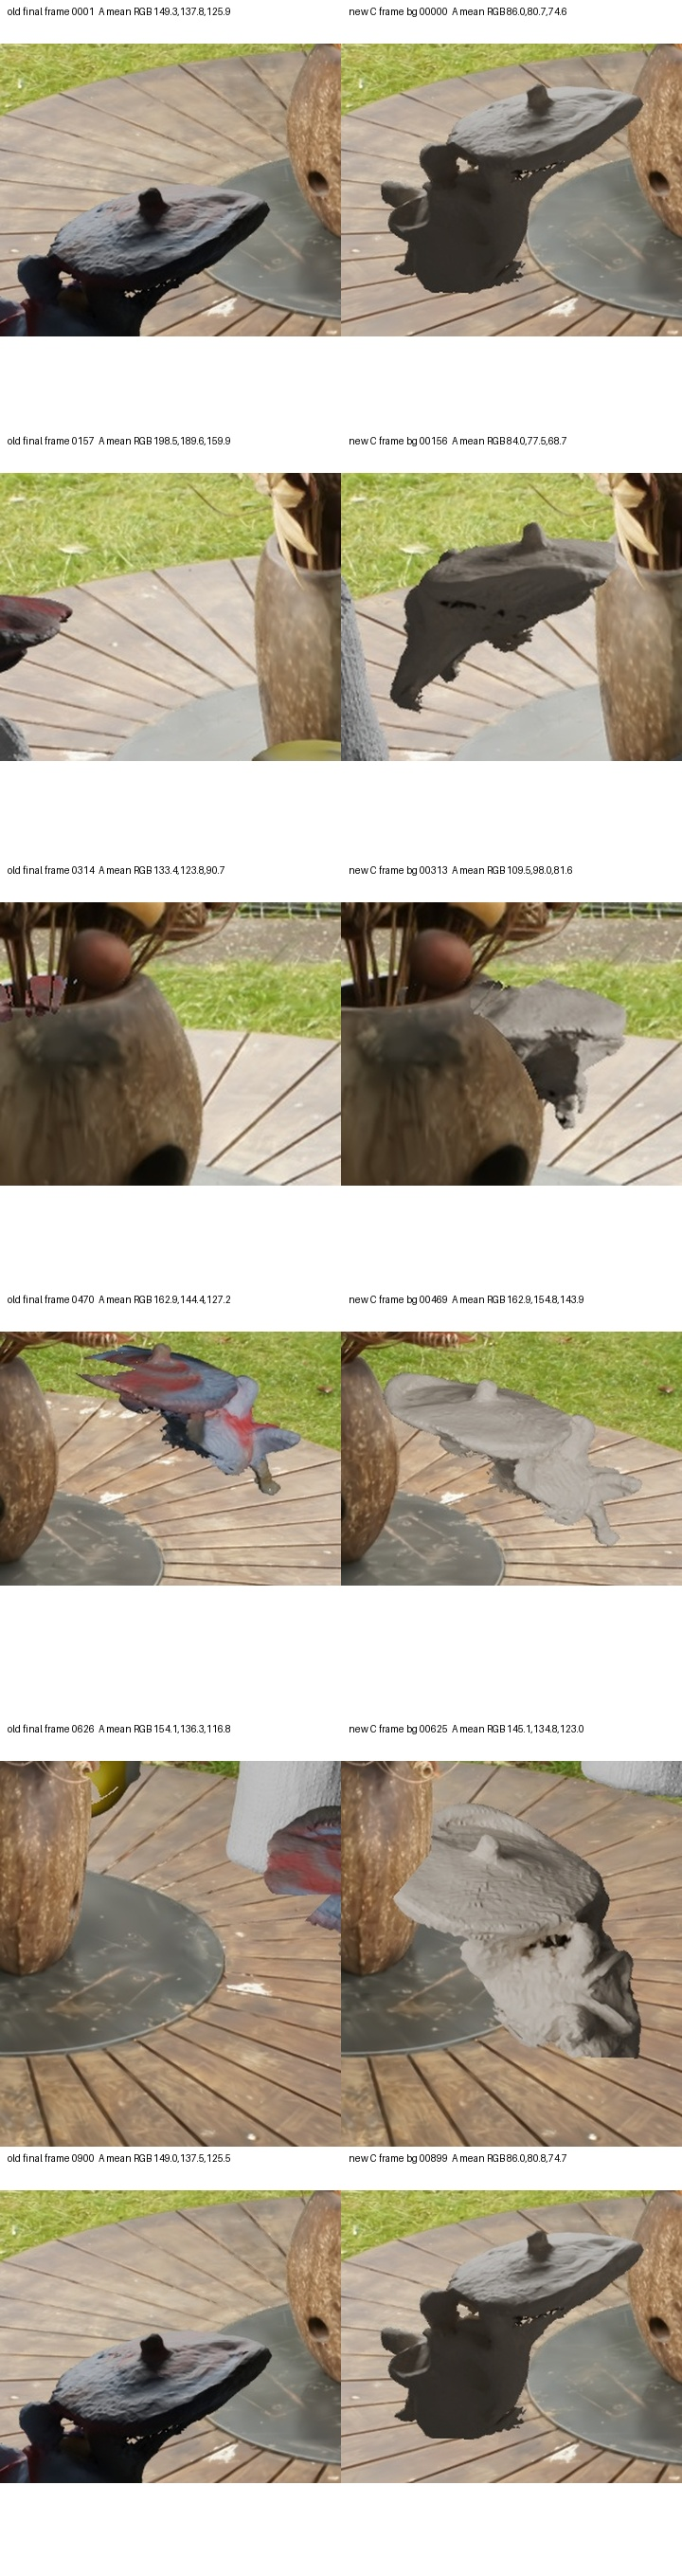
\includegraphics[width=\textwidth,height=0.33\textheight,keepaspectratio]{reports/figures/object_a_old_final_vs_new_mouse_c_color_compare.jpg}
\caption{Object A color and material regression evidence. The left samples use the old accepted final foreground, while the right samples rerender the same old A through the current Blender foreground path and lose the red/blue appearance. This supports the conclusion that A is usable in the accepted foreground but fragile after mesh/material rerendering.}
\label{fig:a_color_regression_appendix}
\end{figure*}

\subsection{Object B SDS Artifacts}
Object B demonstrates prompt sensitivity.
The simple prompt gives richer color but more surface noise and ghosting.
The detailed prompt is not automatically better; it produces blurrier geometry and export instability.
The style-constrained prompt reduces extra-object and Janus risks, so it is selected despite neutral texture.
This supports the final comparison: text-to-3D is flexible, but fidelity is prior-driven rather than observation-driven.

\subsection{Object C Single-image Ambiguity}
Object C is the clearest single-image failure case.
The original Object C experiment used a toy-like input and tested raw image, automatic background removal, and refined mask.
At first, the auto-mask run looked like the best compromise because the front-facing validation views preserved the object identity better than the raw or refined alternatives.
After inspecting the full validation sequence and fused previews, this interpretation was too optimistic.
All three original C variants are rejected as reliable 3D reconstructions.
Table~\ref{tab:c_failure_appendix} records the final post-review scores.

\begin{table}[!htbp]
\centering
\caption{Post-review Object C failure summary. Scores use the same 1--5 rubric as the main experiments, but all first-round C variants are rejected after multi-view inspection.}
\label{tab:c_failure_appendix}
\resizebox{\linewidth}{!}{
\begin{tabular}{lrrrl}
\toprule
Variant & Vert. & Geo & Fusion & Final claim \\
\midrule
Raw image & 18695 & 2 & 1 & background pollution and unstable hidden geometry \\
Auto-mask & 25874 & 1 & 1 & front recognizable, side/back reconstruction failed \\
Refined mask & 27090 & 1 & 1 & cleaner mask, but inflated and fragmented geometry \\
\bottomrule
\end{tabular}
}
\end{table}

The reason is geometric observability.
A single image constrains only the visible projection, not the full surface.
Let $I_c$ be the input image and $S$ be the unknown 3D surface.
Magic123 optimizes a surface whose rendered views are plausible under image and diffusion priors, but there are many surfaces $S'$ that share the same visible front projection:
\begin{equation}
    \Pi_{\mathrm{front}}(S') \approx \Pi_{\mathrm{front}}(S),
    \qquad
    S'_{\mathrm{back}}, S'_{\mathrm{side}} \ \text{unobserved}.
\end{equation}
The back, side thickness, bottom contact surface, and texture atlas structure are therefore prior-driven.
Changing the mask changes not only texture cleanliness but also the feasible silhouette and the surface regularization path.
Raw input pollutes the texture with background; refined mask reduces pollution but worsens side inflation; auto-mask keeps the front appearance but still fails on unseen views.
This explains why a result can look acceptable in a contact sheet row yet fail when placed in the garden: scale, contact, and side-view consistency expose the hidden-surface errors.

The replacement mouse C keeps the same single-image-to-3D route but changes the input object to a simpler, lower-profile shape.
The new Magic123 mesh has 23019 vertices and 46038 faces.
It does not solve the theoretical ambiguity, but it reduces the visible damage because the mouse silhouette is less structurally ambiguous than the original toy and because the final placement exposes mostly the more reliable oblique-front side.
Figure~\ref{fig:c_old_mouse_appendix} compares the original failed C and the mouse replacement through input, fine RGB, depth, and fusion preview.
The important conclusion is not that single-image generation becomes fully reliable; the conclusion is that its errors can be made less dominant by choosing a simpler object and using conservative scale/orientation.

\begin{figure*}[!tbp]
\centering
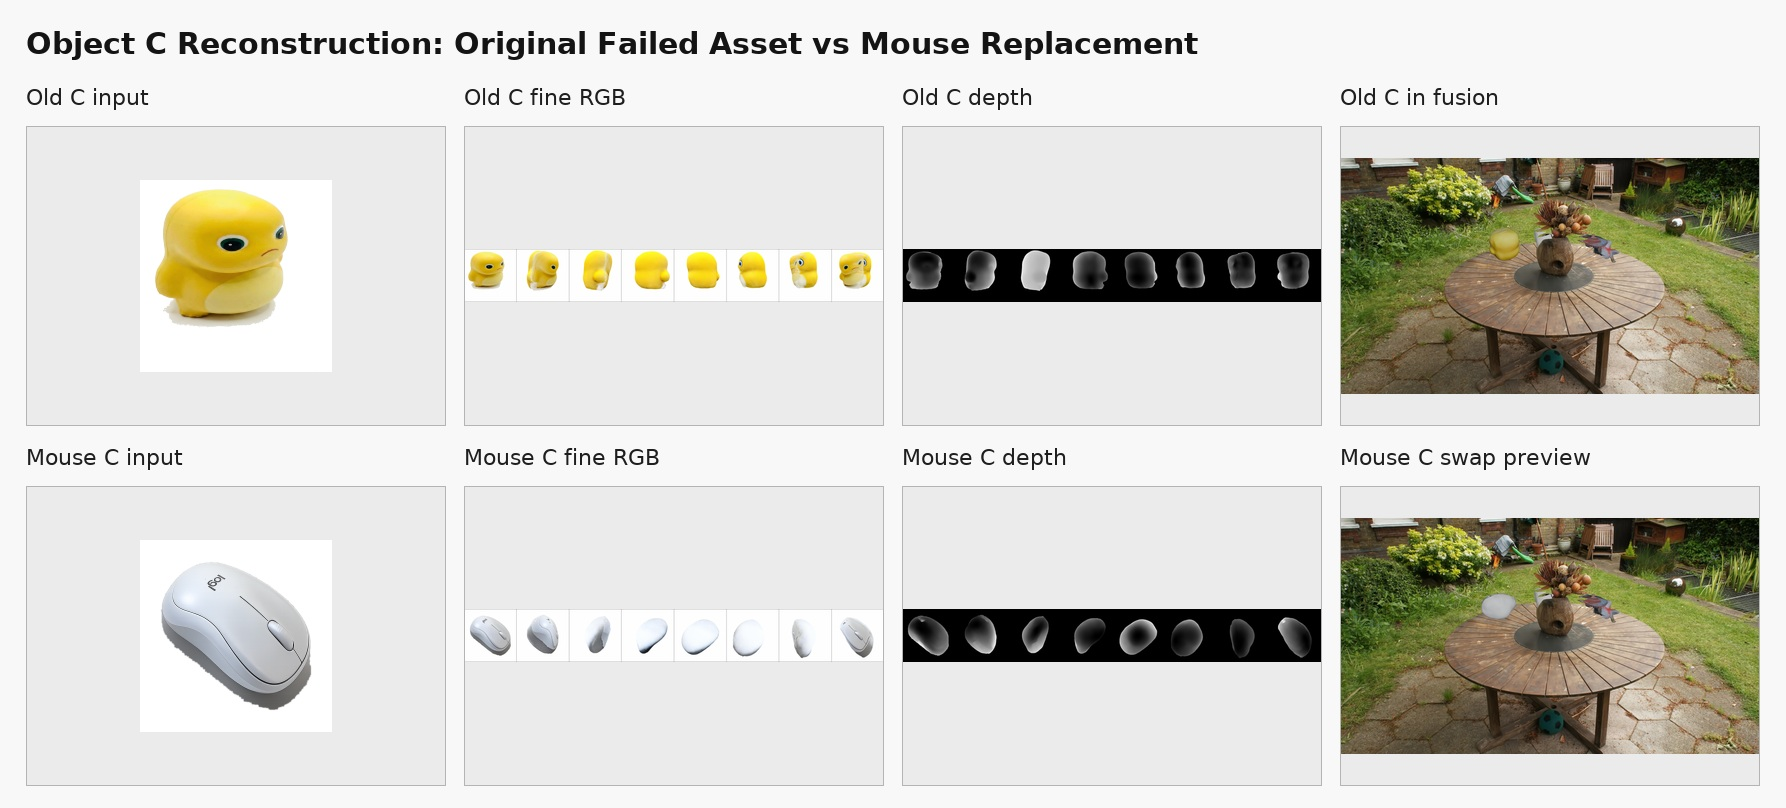
\includegraphics[width=\textwidth,height=0.38\textheight,keepaspectratio]{reports/figures/object_c_old_vs_mouse_reconstruction_comparison.jpg}
\caption{Object C failure and replacement evidence. The original C preserves a front-facing toy appearance but becomes an unreliable yellow object in fusion. The mouse replacement has simpler geometry and a clearer fused silhouette, though its side/back geometry is still inferred from one image.}
\label{fig:c_old_mouse_appendix}
\end{figure*}

\subsection{Gaussian-level Fusion Attempt}
A Gaussian-level extension was tested for Object A by cropping the Object A Gaussian point cloud.
The crop keeps 12067 of 309114 Gaussians, or 3.90\%, and produces a 2.81 MB PLY.
It preserves color and detail in some difficult views, but some views become nearly black because the component-derived bounding box is too conservative.
Figure~\ref{fig:gaussian_crop_appendix} records this smoke test.
The result is useful as an extension but not stable enough for the final mainline.

\begin{figure}[t]
\centering
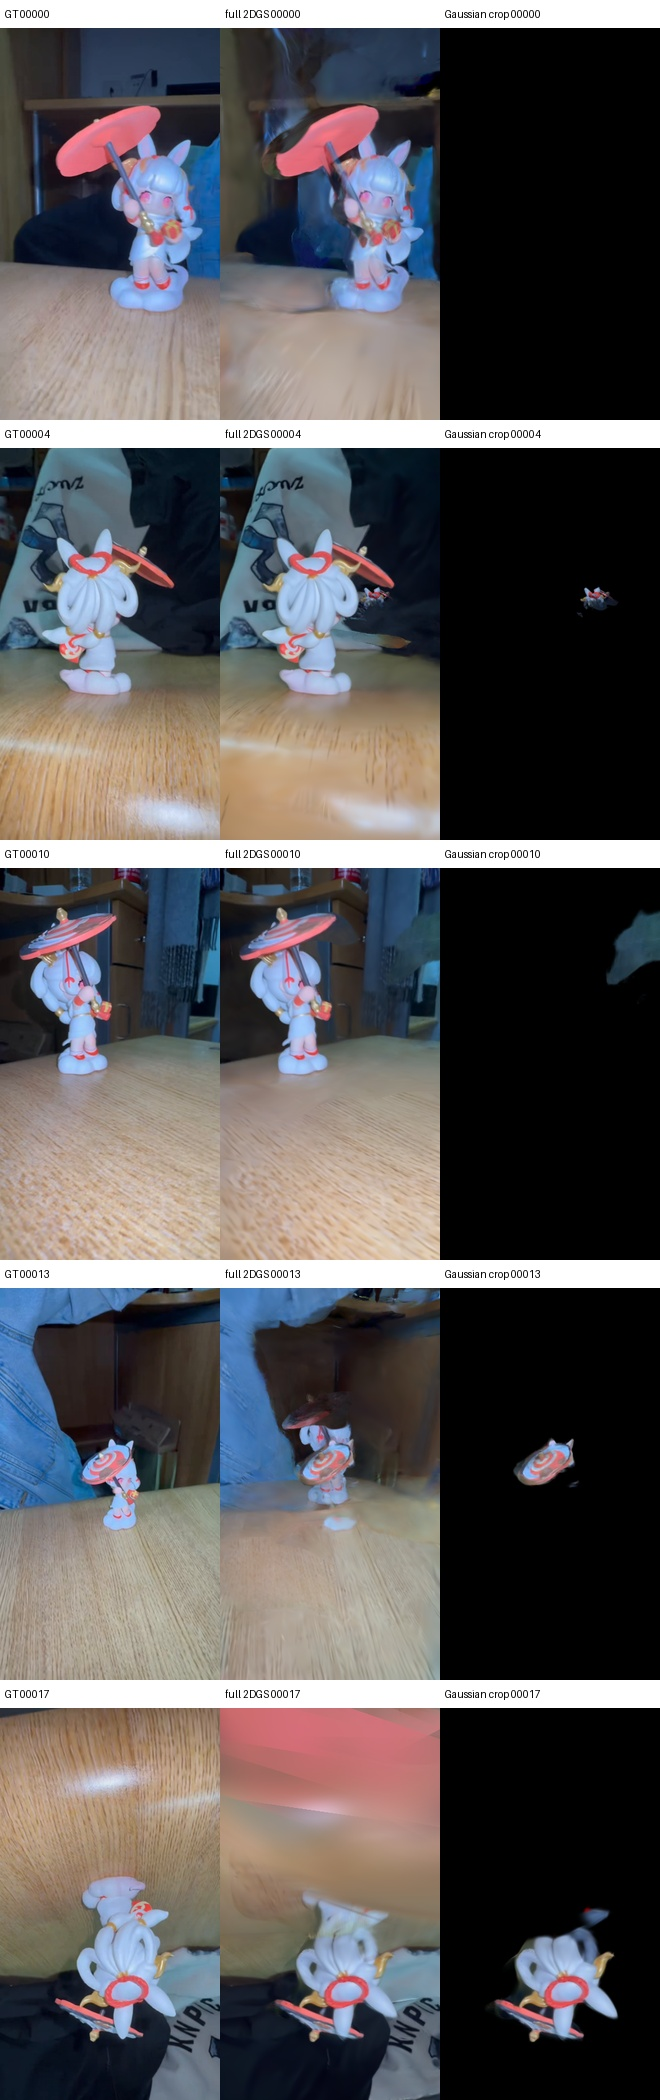
\includegraphics[width=\linewidth,height=0.34\textheight,keepaspectratio]{reports/figures/object_a_gaussian_crop_render_smoke.jpg}
\caption{Gaussian-level Object A crop smoke test. The crop is promising but too sparse in some views, so the final pipeline keeps mesh foreground rendering.}
\label{fig:gaussian_crop_appendix}
\end{figure}

\subsection{Final Video and Error Analysis}
Figure~\ref{fig:final_video_contact} shows that the final video has consistent camera motion across the garden and inserted objects.
The strongest frames show correct table placement and partial occlusion by garden structures.
The weakest frames show image-space depth errors: parts of the background can mask the foreground incorrectly, especially around the vase and thin structures.
This is expected from the compositing inequality in Appendix B.5.
The latest correction also exposes a practical representation issue.
When Object C is replaced, rerendering all A/B/C foreground objects changes Object A's appearance because the current Blender mesh/material path does not reproduce the old accepted A colors.
The final correction therefore uses an image-space C-only swap: old final A/B foreground frames are kept, old C is removed with a C-only alpha mask, and the mouse C foreground is overlaid before the usual 2DGS RGB/depth compositing.
This is not claimed as a physically unified 3D insertion.
It is a controlled correction that preserves the best verified A/B result while replacing the failed C asset.
Fixing it fully would require a true shared 3D representation, such as converting all assets into Gaussian splats and aligning them in the garden COLMAP frame.
The Gaussian crop experiment suggests this is possible, but it also shows that object masking and coordinate alignment are not yet robust enough for the final mainline.

\section{Task 2 Experimental Details}
\todo{Appendix D placeholder for Task 2 experimental details.}

\section{Task 2 Mathematical Formulation}
\todo{Appendix E placeholder for Task 2 mathematical formulation.}

\section{Task 2 Detailed Analysis and Failure Cases}
\todo{Appendix F placeholder for Task 2 detailed analysis and failure cases.}

\section{Submission Links and Artifacts}
\begin{itemize}[leftmargin=*]
    \item GitHub repository: [GitHub URL placeholder]
    \item ModelScope / weights link: [ModelScope URL placeholder]
    \item Final Task 1 video: \figpath{runs/scene/final\_video\_900f\_1080p/final\_scene\_fusion\_15s\_60fps\_1080p.mp4}
    \item Final Task 1 contact sheet: \figpath{reports/figures/final\_scene\_fusion\_900f\_1080p\_contact.jpg}
\end{itemize}

\end{document}
